%% =====================================================================
%%  International Journal of Systems Science: Operations & Logistics
%%  Taylor & Francis "Interact" layout, APA reference style.
%%
%%  interact.cls must sit in the working folder alongside this file and
%%  IJSSOL_CSLAP_v1.bib.
%%
%%  References use BibTeX via apacite (natbibapa); bibliographystyle is
%%  set to apacite below. Do not also load natbib.
%% =====================================================================
% Ensure the "table" option reaches xcolor no matter which package pulls it in
% first (tikz also loads xcolor); this avoids an option clash.
\PassOptionsToPackage{table}{xcolor}
\documentclass[]{interact}

% interact.cls already loads amsmath, amssymb, amsfonts, amsthm, booktabs,
% epsfig, graphicx and rotating. We add only what this manuscript needs.
\usepackage{mathtools}
\usepackage{multirow}
\usepackage{float}
\usepackage{xcolor}  % "table" option passed above; enables \rowcolor/\cellcolor
\usepackage{algorithmicx}
\usepackage{algorithm}
\usepackage{algpseudocode}
\usepackage{tabularx}
\usepackage{colortbl}
\usepackage{xltabular}



% Removes vertical gaps introduced by booktabs around colored rows
\setlength{\aboverulesep}{0pt}
\setlength{\belowrulesep}{0pt}

\usepackage{booktabs}
\usepackage{tikz}
\usetikzlibrary{shapes.geometric, arrows.meta, positioning, calc}
\usepackage{url}
\usepackage{hyperref}

% APA references via BibTeX, exactly as the interact-APA sample documents.
\usepackage[natbibapa,nodoi]{apacite}
\setlength\bibhang{12pt}
\renewcommand\bibliographytypesize{\fontsize{10}{12}\selectfont}

\begin{document}

\articletype{RESEARCH ARTICLE}

\title{Minimising station visits in automated pick-and-pass warehouses: a correlated storage assignment model validated at industrial scale}

\author{
\name{Ermal Belul\textsuperscript{a,b}\thanks{CONTACT Ermal Belul. Email: ermal.belul@hds.utc.fr. Co-author emails: Marwane Bouznif marwane.bouznif@savoye.com, Dritan Nace dritan.nace@hds.utc.fr, Antoine Jouglet antoine.jouglet@hds.utc.fr. ORCID: Ermal Belul 0009-0006-3589-6267, Marwane Bouznif 0000-0002-5138-1582, Dritan Nace 0000-0003-3914-2463, Antoine Jouglet 0000-0001-9251-249X.},
Marwane Bouznif\textsuperscript{b},
Dritan Nace\textsuperscript{a} and
Antoine Jouglet\textsuperscript{a}}
\affil{\textsuperscript{a}Universit\'{e} de technologie de Compi\`{e}gne, CNRS, Heudiasyc UMR 7253, Compi\`{e}gne, France; \textsuperscript{b}Savoye, France}
}

\maketitle

% ---------------------------------------------------------------------
% Unstructured abstract (<= 200 words, single paragraph)
% ---------------------------------------------------------------------
\begin{abstract}
In automated pick-and-pass warehouses the conveyor carries each order past fixed stations, so the operational cost driver is the number of stations an order visits rather than picker travel distance. Correlated storage models nonetheless inherit distance-minimisation objectives from manual picking. We reformulate it to minimise station visits subject to hard per-station slot capacity and workload budgets. The objective is piecewise constant, since an order's visit count changes only when it gains or loses a whole station, so most single-product moves leave it unchanged, and the linear relaxation is too weak to guide branch-and-bound. We build three strategies around that structure: a set-variable formulation, a set-partitioning column generation, and a clustering heuristic. Across 29 benchmark instances under one protocol, all three return fewer visits than a genetic algorithm and simulated annealing taken as literature baselines, the margin widening with catalogue size under the size-dependent budgets tested. Applied to an operating facility with 21,874 products and 26 picking stations, the set-variable formulation removes 13.7\% of station visits in sample and 6.6 to 7.4\% on held-out weeks, every station remaining inside its workload budget. A bounded reassignment extension shows how much of that gain a capped relocation budget recovers, for adoption in stages.
\end{abstract}

\begin{keywords}
storage location assignment; pick-and-pass warehouse; warehouse automation; mixed-integer programming; column generation; metaheuristics
\end{keywords}


% =====================================================================
\section{Introduction}
% =====================================================================
Order picking absorbs a large share of warehouse operating cost, so where products sit on the shelves has a direct effect on throughput \citep{xie2024combi}. The correlated storage location assignment problem (CSLAP) chooses that placement by grouping products frequently ordered together, and most CSLAP models pursue that aim by minimising picker travel distance \citep{islam2023}. That objective suits a warehouse where a picker walks the aisles, not one where goods move on a conveyor. In an automated pick-and-pass facility the movement of totes between zones is mechanised, and the binding limit is how often a tote leaves the main line and merges back into it: each diversion adds a fixed mechanical and handling delay and occupies a slot in a finite station buffer, so the cost driver becomes station visits per order together with the balance of workload across zones. We build a CSLAP model on that basis, with total station visits as the objective and no station permitted to exceed its physical capacity or workload budget.

Solving that model at the scale of a real warehouse is difficult for two reasons. The objective counts discrete stops, so its value changes only when a whole order gains or loses a zone and relocating a single product usually leaves it unchanged, so a search steered by the visit count spends most of its moves on a plateau. On the instance family studied here the linear relaxation of the binary programme is meanwhile no stronger than the observation that every order visits at least one station, whatever the correlation structure (Supplementary Section~S6), so branch-and-bound starts from a root bound carrying nothing instance-specific to prune with.

We make three contributions. First, we pose CSLAP for pick-and-pass systems with station visits as the objective under hard per-station capacity and workload limits, replacing the travel-distance objective the correlated storage literature inherits from manual picking, and give the model in two equivalent forms, a binary encoding and a set-variable reformulation (Section~\ref{sec:model}). Second, we show how the structure of that objective shapes the solution space and build three complementary strategies around it: a set-variable formulation, in which single-station assignment is a property of the representation rather than a constraint the search must repair; a set-partitioning column generation, whose unit of change is a whole product bundle rather than one product; and a clustering heuristic that works on the correlation graph directly. The binary encoding is retained as a representation control, and a genetic algorithm (GA) and simulated annealing with correlated interchange (SA-C) provide the external comparison over 29 instances under one protocol with paired tests (Sections~\ref{sec:methods} and~\ref{sec:experiments}). Third, we validate the model on a real warehouse of 21,874 products and 26 stations, where the reduction holds on weeks the layout was not fitted to and every station stays inside its own workload budget, and add a bounded reassignment extension capping how many products may move, so the gain deploys gradually on an active facility (Section~\ref{sec:industrial}).

% =====================================================================
\section{Related work}\label{sec:litreview}
% =====================================================================
In a manual warehouse a picker walks to the shelves, so preparation time follows the distance walked and storage models minimise it \citep{islam2023, wang2020}. \citet{zhang2019cie} model demand correlation explicitly and place co-ordered products near a depot, and \citet{xiao2010correlated} use bill-of-material structure to the same end, again measuring the benefit in distance saved. That objective does not describe an automated pick-and-pass warehouse, where a conveyor carries the order past fixed stations and no picker travel occurs. Where goods move mechanically the limits are instead station visits, order splits, mechanical dwell and the synchronisation of workload across zones \citep{azadeh2019, xie2021}, all originating in the per-diversion setup and in the queueing of finite station buffers, both of which fall when an order visits fewer zones \citep{zhu2021, kim2020}. \citet{dekoster2012zones} set the number of zones in a pick-and-sort system by minimising batch completion time; their decision fixes how many zones there are, ours their content.

Three recent models optimise these discrete interactions directly. \citet{zhu2021} minimise order splits across multiple warehouses by clustering, which maps to grouping products into conveyor zones so an order stays intact. \citet{xie2021} minimise pod-station visits, the delivery of one movable shelf rack to one station and the analogue of our station visit, and prove that fewer visits with dispersed workload raise throughput. \citet{mirzaei2021} propose correlated dispersed storage, spreading correlated items across automated assets to avoid a queue at any single workstation. Reducing visits must therefore be paired with workload balance, modelled explicitly: \citet{tarczynski2023} show balance is a precondition for reducing picking time in pick-and-pass zones, \citet{vanGils2018} show storage assignment and zoning must be optimised together, and \citet{boysen2023} conclude that delivering each tote to a capacity-feasible station without queueing is the main determinant of throughput. Whether balance enters the objective or the constraints is itself a choice: \citet{saylam2023minmax} minimise the maximum completion time across zones, whereas \citet{vanheusden2022workload} find the appropriate measure depends on the managerial reason for balancing rather than the layout. We place the limit in the constraints because each station on an installed conveyor has an engineered daily budget operations treat as hard, so the question is not how evenly work is spread but how few visits are reachable without exceeding it.

Storage assignment under hard synchronisation carries the structure of a constrained partitioning problem for which no polynomial method is known, and decomposition methods have gained ground on it. \citet{muter2022} solve a set-partitioning model of order batching and picker scheduling by column generation with workload pacing inside pricing, and \citet{zhen2025} design column-and-row generation for hard synchronisation in autonomous-robot warehouses; station capacity and workload can therefore be carried as resource limits inside a pricing subproblem, the route we follow. Two known difficulties shape our design: a per-order coverage encoding makes pricing scale with the raw order count, and a station-indexed master over identical stations is invariant under relabelling, a symmetry degrading both the relaxation and the integer search \citep{vanderbeck2000dw}. Our framework prices over distinct weighted order supports and, when stations are interchangeable, aggregates the master so the symmetry never arises. Degeneracy of the covering master is a further difficulty our design does not address: it is usually met with dual stabilisation \citep{dumerle1999stabilized, wentges1997weighted}, and we report where it would help rather than implementing it.

Adaptive large neighbourhood search \citep{ropke2006alns} and open-source constraint programming over Boolean satisfiability \citep{perron2023cpsat} are closely related paradigms that Section~\ref{sec:conclusion} returns to as the comparisons this study does not make, while learning-based hybrids such as \citet{barnhart2024learnthenoptimize} schedule operations over a short horizon, whereas our decision is the strategic placement those operations inherit. Table~\ref{tab:litreview} positions this paper along the dimensions that matter in the automated setting: several authors already advocate the visit objective, but to our knowledge no study solves it for a real catalogue of tens of thousands of products under hard per-station workload limits, validated on an operating facility.

\begin{table}[H]
\centering
\tbl{Positioning of this study against representative storage-assignment and order-picking research.}
{\footnotesize\setlength{\tabcolsep}{3pt}
\begin{tabularx}{\textwidth}{@{}l X c X X >{\raggedright\arraybackslash}p{2.8cm}@{}}
\toprule
Study & Objective & Hard WL cap & Setting & Largest instance & Method \\
\midrule
\citet{zhang2019cie}        & Travel distance       & No    & Manual, correlated      & Hundreds of SKUs & MILP, heuristic \\
\citet{wang2020}            & Travel distance       & No    & Manual picker-to-parts  & Hundreds of SKUs & Clustering \\
\citet{dekoster2012zones}   & Completion time       & No    & Pick-and-sort zoning    & Not stated & Analytical, heuristic \\
\citet{mirzaei2021}         & Dispersion/affinity   & Partial & Robotic fulfilment   & $\sim 10^3$ SKUs & MIP, policy \\
\citet{xie2021}             & Pod-station visits    & No    & Robotic fulfilment      & $\sim 10^3$ items & MIP \\
\citet{tarczynski2023}      & Picking time          & Yes   & Pick-and-pass           & Small to medium & LP, MILP \\
\citet{vanheusden2022workload} & Workload balance    & Yes   & Manual zone picking   & Not stated & Iterated local search \\
\citet{saylam2023minmax}    & Makespan (min--max)   & Yes   & Dynamic zone picking    & Not stated & MILP, dynamic prog. \\
\citet{muter2022}           & Makespan              & Yes   & Batching/picking        & Medium & Column generation \\
This study                  & Station visits        & Yes   & Pick-and-pass, automated & 21,874 real SKUs & Set-variable form., CG, heuristic \\
\bottomrule
\end{tabularx}}
\tabnote{WL cap: whether a hard per-station workload limit is enforced; ``Partial'' denotes a soft or aggregate limit. CG: column generation. ``Not stated'' indicates the source reports no instance size.}
\label{tab:litreview}
\end{table}



% =====================================================================
\section{Problem definition and decision-aid model}\label{sec:model}
% =====================================================================
%\subsection{The pick-and-pass picking section}
Orders travel along a main conveyor and pass a sequence of picking stations, each on a spur off the main line (Figure~\ref{fig:schematic}) and each holding a fixed set of products on nearby shelving. When an order needs a product stored at a station its tote diverts onto the spur, an operator picks the required items, and the tote merges back, repeating this at every station holding one of its products before leaving for dispatch. One such diversion is a \emph{station visit}, and an \emph{order split} occurs when an order's products sit across more than one station.

\begin{figure}[H]
\centering
\resizebox{\textwidth}{!}{%
\begin{tikzpicture}[
  font=\small,
  station/.style={draw, rounded corners, fill=blue!8, minimum width=1.9cm, minimum height=0.95cm, align=center},
  bin/.style={draw, fill=orange!30, minimum size=0.30cm, inner sep=0pt},
  conv/.style={line width=2pt, -{Latex[length=3mm]}, black!70},
  spur/.style={thick, -{Latex[length=2mm]}, gray!60!black},
]
\draw[line width=6pt, gray!20] (-0.2,0) -- (12.2,0);
\draw[conv] (-0.2,0) -- (12.6,0);
\node[left] at (-0.3,0) {Input};
\node[right] at (12.7,0) {Dispatch};
\node[below, font=\footnotesize] at (6.2,-0.28) {Main conveyor (orders advance in sequence)};
\node[station] (s1) at (2.4,2.25) {Station $s_1$};
\node[station] (s2) at (6.2,2.25) {Station $s_2$};
\node[station] (s3) at (10.0,2.25) {Station $s_{|S|}$};
\node[font=\scriptsize] at (8.2,2.25) {$\cdots$};
\foreach \x in {2.4,6.2,10.0}{
  \draw[spur] (\x-0.65,0.05) -- (\x-0.65,1.75);
  \draw[spur] (\x+0.65,1.75) -- (\x+0.65,0.05);
}
\node[font=\scriptsize, gray!50!black, align=center] at (2.4,1.0) {divert $\uparrow$\\ merge $\downarrow$};
\foreach \x in {0.5,1.4,4.3,8.0,11.4}{ \node[bin] at (\x,0) {}; }
\node[font=\scriptsize, orange!60!black] at (0.5,-0.55) {order tote ($P_o$)};
\node[bin] at (5.55,0.5) {};
\node[bin] at (5.55,0.86) {};
\node[align=center, font=\scriptsize] at (6.2,0.95) {finite\\ buffer};
\draw[step=0.27cm, gray!55, thin] (1.45,2.95) grid (3.35,3.4);
\node[font=\scriptsize] at (2.4,3.62) {shelving: products stored at $s$};
\end{tikzpicture}%
}
\caption{A pick-and-pass picking section: a tote diverts onto a station's spur whenever that station stores one of the order's products $P_o$, and each diversion counts as one station visit.}
\label{fig:schematic}
\end{figure}

Two operational facts drive the model. A visit carries a fixed cost independent of how many items are picked, because the tote must still be decelerated, inducted, scanned and merged, so grouping co-ordered products at one station collects more items per stop and lowers the visit count. It also decongests the finite station buffer, whose overflow blocks the main line: a station calibrated for 1,000 lines a day handles 500 totes if it serves 500 two-line orders, but only 200 for the same picking work in five-line orders. The model does not observe diversion traffic directly, so holding a station's assigned lines within its engineered daily budget serves as the operational proxy. Both effects are captured below, visits in the objective and workload in a hard constraint.

\subsection{Sets, parameters, decisions, and the mixed-integer linear programme}
Let $P$ be the catalogue of products, each one stock-keeping unit (SKU), $O$ the orders observed over the planning horizon, and $S$ the stations. Order $o$ requests the products of its line set $P_o \subseteq P$, and $L_p$ is the number of order lines in which product $p$ occurs. Each station $s$ has $\zeta_s$ storage locations, a processing rate $V_s$ in lines per unit time, and a workload budget $T_s$ in the units of $\sum_{p} L_p/V_s$; the product $C_s := T_s V_s$ is its line capacity, the form the pricing subproblem of Section~\ref{sec:cg} uses. We model placement at the station level, assigning a product to exactly one station without fixing which physical slot it occupies, since shelving can be rearranged without changing $\zeta_s$; duplication is left to Section~\ref{sec:conclusion}. Supplementary Section~S10 collects the notation.

We present the model in two equivalent forms. The first uses the standard binary encoding below, whereas the second replaces the binary matrix with set decision variables, an abstraction specific to the Hexaly solver \citep{blaisemodeling} that exposes high-level partition operators to the search (Section~\ref{sec:setvar}). Both encode the same assignment problem. The binary variable $x_{ps}$ is 1 when product $p$ is assigned to station $s$, and $z_{os}$ records whether order $o$ visits station $s$, forced to 1 whenever any product of $o$ sits at $s$. The model is
\begin{align}
\min \quad & \sum_{o \in O} \sum_{s \in S} z_{os} \label{eq:obj}\\
\text{s.t.} \quad
& \sum_{s \in S} x_{ps} = 1 && \forall p \in P \label{eq:assign}\\
& \sum_{p \in P} x_{ps} \le \zeta_s && \forall s \in S \label{eq:cap}\\
& x_{ps} \le z_{os} && \forall o \in O,\ p \in P_o,\ s \in S \label{eq:link}\\
& \sum_{p \in P} x_{ps}\,\frac{L_p}{V_s} \le T_s && \forall s \in S \label{eq:wl}\\
& x_{ps} \in \{0,1\},\quad z_{os} \in [0,1]. && \label{eq:dom}
\end{align}
Three points are not evident from the rows. (i) The objective drives $z_{os}$ to its lower bound, so it takes value 1 only when a visit is unavoidable and stays integral without a big-$M$ term despite being declared continuous. (ii) In the workload cap \eqref{eq:wl} the sum runs over all products assigned to the station, not over a single order. (iii) Summing the linking rows \eqref{eq:link} over the stations gives $\sum_{s} z_{os}\ge 1$ for every order, a floor $x_{ps}=1/|S|$ attains under the operational slack of Section~\ref{sec:experiments}, so on this family the linear relaxation is worth exactly $|O|$ whatever the correlation structure (Supplementary Section~S6).

\subsection{Set-variable reformulation}\label{sec:setvar}
The same model admits an alternative representation through set decision variables, a feature of the Hexaly solver that replaces the binary assignment matrix with one set variable per station \citep{blaisemodeling}, whose high-level operators (partition, contains, count) let the solver navigate the flat, step-function landscape without flipping individual binary flags. The set variable $\Phi_s$ holds the subset of products assigned to station $s$, so $\{\Phi_s\}_{s \in S}$ replaces the matrix $x_{ps}$ and the number of declared variables falls from $|P|\times|S|$ to $|S|$. The model reads
\begin{align}
\min \quad & \sum_{o \in O} \bigl|\{\, s \in S \,:\, \Phi_s \cap P_o \neq \emptyset \,\}\bigr| \label{eq:setobj}\\
\text{s.t.} \quad & \{\Phi_s\}_{s \in S}\ \text{is a partition of}\ P, \label{eq:setpart}\\
& |\Phi_s| \le \zeta_s && \forall s \in S, \label{eq:setcap}\\
& \sum_{p \in \Phi_s} L_p / V_s \le T_s && \forall s \in S, \label{eq:setwl}
\end{align}
where \eqref{eq:setobj} counts, for each order, the stations holding at least one of its products, the value $\sum_{s} z_{os}$ takes at optimality in \eqref{eq:obj}, and \eqref{eq:setcap} and \eqref{eq:setwl} restate \eqref{eq:cap} and \eqref{eq:wl} on the partition. Only the representation changes, and the problem is hard either way: setting the visit objective aside, the slot-capacity rows alone ask for a partition of the catalogue into $|S|$ blocks of bounded size under a bounded per-block load, the structure of multiway number partitioning \citep{garey1979computers}, so we expect no polynomial method and claim no reduction here. What changes is the burden on the search: \eqref{eq:assign} is not written at all, since a partition satisfies it by construction, so single-station assignment becomes a property of the representation rather than something the search must repair. We solve both forms with Hexaly and call them the binary MILP and the set-variable formulation; on a few thousand products the two perform alike, and the reformulation separates only at industrial scale (Section~\ref{sec:industrial}).

% =====================================================================
\section{Solution methods}\label{sec:methods}
% =====================================================================
Three solution strategies address the model, and the binary encoding of Section~\ref{sec:model} runs alongside them as a representation control rather than as a fourth strategy. All of them minimise station visits subject to the slot capacity~\eqref{eq:cap} and the workload cap~\eqref{eq:wl}, and differ in what they give up to do it. The binary and set-variable forms consume the largest budget and are compared against each other on the same engine under the same cap, which isolates the effect of the decision representation while holding the search technology fixed. The clustering heuristic returns a feasible layout in minutes with no certificate of quality, whereas the set-partitioning column generation searches at the level of whole product bundles and returns a stream of feasible layouts with a lower bound it reports as a diagnostic. The GA and SA-C baselines of Section~\ref{sec:baselines} provide the external comparison.

\subsection{Fast feasible layouts: greedy clustering heuristic}\label{sec:heuristic}
For catalogues of this size we use a fast heuristic that groups strongly co-ordered products into communities and places them on stations under both capacity constraints, extending the agglomerative idea of \citet{chuang2016} but building disjoint communities by greedy graph connectivity. Three thresholds filter the correlation graph and a fourth bounds the communities built on it. The filters are indexed on catalogue volume $N=|P|$, so a pair count that signals affinity at 50 products is noise at 20,000, whereas the bound is indexed on the slot capacity of a station, because a community must fit inside one. That fourth rule therefore presumes the stations are alike; where capacities differ widely no single number describes the room any of them has, and Section~\ref{sec:industrial} reports what it costs on such a site.
\begin{itemize}
\item $\phi=\max(2,\lfloor N/100\rfloor)$, the frequency floor: a product enters the graph only if it appears in at least $\phi$ orders, anchoring the noise floor at 1\% of catalogue volume.
\item $\gamma=\max(2,\lfloor N/50\rfloor)$, the co-occurrence floor: a pair enters only if its products are ordered together at least $\gamma$ times.
\item $r=0.1$, the kept-edge ratio: a pair survives only if its co-occurrence reaches a tenth of the more frequent endpoint's own demand, removing edges inflated by one ubiquitous endpoint.
\item $\beta=\max\!\left(5,\big\lfloor 0.4\,\zeta+\tfrac12 \big\rfloor\right)$, the community size bound, where $\zeta=|P|/|S|$ is the slot capacity of a station: it prevents clusters no station can hold.
\end{itemize}
The coefficient $0.4$ is calibrated on a separate family of 80 instances built so the same $\zeta$ occurs at two catalogue sizes, which the benchmark of Section~\ref{sec:experiments} cannot do because its generator ties the station count to the catalogue. Across its eight geometry cells the visit-minimising bound $\beta^\ast$ is identical at both catalogue sizes for a fixed slot capacity and moves with $\zeta$ across the whole range for a fixed catalogue, the Spearman rank correlation between $\beta^\ast$ and $\zeta$ being $1.000$ against $0.000$ between $\beta^\ast$ and $N$ (Supplementary Section~S1). The dependence is monotone but not proportional, the minimising ratio being $0.60$ at $\zeta\le 50$ and $0.40$ at $\zeta=100$, the capacity of every benchmark instance of 500 SKUs and above; we adopt $0.4$ because it minimises at the sizes the method is intended for and errs low elsewhere, where larger communities are harder to place within the workload constraint. It is deliberately not optimal at the smallest size, where $\zeta=10$ puts the bound on its floor of 5 and the coefficient plays no role, leaving the heuristic's $+6.9\%$ gap there a property of the method rather than this threshold. Supplementary Section~S2 rescales all four thresholds and finds the response shallow, so we keep the defaults and tune none per instance.

Figure~\ref{fig:heuristic_flow} gives the five stages. At placement a community goes to the station with room for it whole that already holds the largest share of its products in the incumbent layout, ties settled towards the lower load ratio, the incumbent being the live layout on the industrial case and the longest-processing-time (LPT) start of Section~\ref{sec:init} on the synthetic instances; a community fitting nowhere whole is split. Supplementary Section~S4 states the procedure as pseudocode.

The last stage repairs workload by exchanging products rather than relocating them, because there is nowhere to relocate to: the benchmark instances give $\sum_s \zeta_s = |P|$ exactly and on the industrial site each station's capacity is the number of products it already holds, so an exchange leaves both product counts unchanged while moving only the workload. Write $\mathrm{cnt}_{xy}$ for the number of orders containing both products $x$ and $y$, $\mathrm{load}(s)=\sum_{p\in s}L_p/V_s$ for the workload of station $s$, and $A(x,C)=\sum_{y\in C}\mathrm{cnt}_{xy}$ for the co-occurrence weight tying a product $x$ to the products of a set $C$, which measures how strongly $x$ belongs with what $C$ already holds. The stage repeatedly takes the station $s$ of greatest relative overload $\mathrm{load}(s)/T_s$ and exchanges one of its products $p$ against a product $q$ of another station $t$, drawing $p$ from the products of $s$ of largest $L_p$ and $q$ from those of $t$ of smallest $L_q$, and admitting only exchanges with $L_q < L_p$ that leave $t$ inside its own cap. Among those it applies the one breaking the least co-occurrence weight,
\[
\Delta_{\mathrm{aff}}=A(p,s\setminus\{p\})+A(q,t\setminus\{q\})-A(p,t\setminus\{q\})-A(q,s\setminus\{p\}),
\]
each exchanged product being removed from the set it is scored against, since neither stays where it was. The loop stops when every station is inside its cap, when no admissible exchange remains, or when a cap of $10|P|+100$ exchanges is reached; the last two are termination conditions rather than feasibility guarantees, and every run reported here ended with no station over its cap.

\begin{figure}[H]
\centering
\resizebox{0.92\linewidth}{!}{%
\begin{tikzpicture}[
  font=\small,
  node distance=1.1cm and 1.5cm,
  startstop/.style={rectangle, rounded corners, minimum width=3.5cm, minimum height=1cm, text centered, draw=black, fill=red!10},
  process/.style={rectangle, minimum width=4cm, minimum height=1cm, text centered, draw=black, fill=blue!10, align=center},
  decision/.style={diamond, aspect=2, minimum width=3.5cm, minimum height=1cm, text centered, draw=black, fill=green!10, align=center},
  arrow/.style={thick, -{Latex[length=3mm]}}
]
\node (start) [startstop] {Input data ($P,O$) and thresholds};
\node (preproc) [process, below=1cm of start] {\textbf{Step 1: preprocessing}\\filter noise, form valid pairs};
\node (initcomm) [process, below=1cm of preproc] {Initialise community set $\mathcal{C} \leftarrow \emptyset$};
\node (decide1) [decision, below=1cm of initcomm] {Candidate\\pairs left?};
\node (form) [process, right=2cm of decide1] {\textbf{Step 2: community formation}\\greedy expansion of the top pair\\up to the size bound};
\node (post) [process, below=1cm of decide1] {\textbf{Step 3: post-processing}\\assign residual and low-frequency SKUs};
\node (sort) [process, below=1cm of post] {Rank communities by cumulative demand};
\node (decide2) [decision, below=1cm of sort] {Communities\\unassigned?};
\node (assign) [process, right=2cm of decide2] {\textbf{Step 4: station assignment}\\place or split under $\zeta_s$ \emph{and} the workload cap};
\node (repair) [process, below=1cm of decide2] {\textbf{Step 5: workload repair}\\exchange products until no station is over its\\cap or no admissible exchange remains};
\node (end) [startstop, below=1cm of repair] {Final product-to-station assignment};
\draw [arrow] (start) -- (preproc);
\draw [arrow] (preproc) -- (initcomm);
\draw [arrow] (initcomm) -- (decide1);
\draw [arrow] (decide1) -- node[anchor=south] {yes} (form);
\draw [arrow] (form) |- ($(initcomm.south) + (0,-0.4)$) -| (decide1);
\draw [arrow] (decide1) -- node[anchor=east] {no} (post);
\draw [arrow] (post) -- (sort);
\draw [arrow] (sort) -- (decide2);
\draw [arrow] (decide2) -- node[anchor=south] {yes} (assign);
\draw [arrow] (assign) |- ($(sort.south) + (0,-0.4)$) -| (decide2);
\draw [arrow] (decide2) -- node[anchor=east] {no} (repair);
\draw [arrow] (repair) -- (end);
\end{tikzpicture}
}
\caption{The five stages of the greedy clustering and station-assignment heuristic. Each loop exits when no candidate pair or unassigned community remains.}
\label{fig:heuristic_flow}
\end{figure}

The heuristic is a single-pass, deterministic constructive procedure with no objective-improving local search and no time parameter. One pass takes 1 to 47 seconds across the synthetic benchmarks, rising with the order lines the pair-counting step scans, and 94 seconds on the industrial catalogue. Where the bound has to be searched rather than read off the rule, the search dominates that cost, and Table~\ref{tab:industrial} charges the whole of it.


\subsection{Bundle-level search: set-partitioning column generation with a price-and-complete drive}\label{sec:cg}
The obstacle of Section~\ref{sec:methods} is the unit of change. Station visits move only when a whole order gains or loses a station, so a search that relocates one product at a time usually reads no change, whereas a method whose smallest move is a whole group registers where a single-product move does not. A set-partitioning decomposition supplies that unit: its columns are complete product bundles, each a set a station could hold, and choosing one installs the group in a single step. We build it following large-scale pricing methods for logistics and scheduling \citep{lubbecke2005selected, muter2022}, with a \emph{master problem} choosing among the bundles generated so far and \emph{pricing} searching for a new bundle worth adding.

\subsubsection{Station-indexed and aggregated masters}\label{sec:cgmaster}
The problem decomposes naturally by station. A \emph{pattern} is a set of products a single station could hold, and $K_s$ is the family feasible for station $s$: subsets $q \subseteq P$ with $|q| \le \zeta_s$ and $\sum_{p \in q} L_p / V_s \le T_s$. The \emph{support} of an order is its line set $P_o$. Many orders share a support, so let $U$ be the set of distinct \emph{multi-item} supports, each with weight $w_u$ equal to the number of orders sharing it; singleton orders visit exactly one station under every layout, so singleton supports contribute a layout-independent constant and are excluded from $U$. With one column per station-pattern pair, the pattern cost $c_q = \sum_{u \in U} w_u\,\mathbf{1}[q \cap u \neq \emptyset]$ counts the weighted supports a pattern touches, and the linear master reads
\begin{align}
\min \quad & \sum_{s \in S} \sum_{q \in K_s} c_q\, y_{sq} \notag\\
\text{s.t.} \quad
& \sum_{s \in S} \sum_{q \in K_s:\, p \in q} y_{sq} \ge 1 && \forall p \in P \quad (\sigma_p \ge 0) \label{eq:covergen}\\
& \sum_{q \in K_s} y_{sq} \le 1 && \forall s \in S \quad (\mu_s \le 0) \label{eq:convgen}\\
& 0 \le y_{sq} \le 1 && \forall s \in S,\ q \in K_s. \notag
\end{align}
Constraint \eqref{eq:covergen} covers every product and the convexity rows \eqref{eq:convgen} select at most one pattern per station, with the dual of each family in parentheses. For any integer solution whose patterns partition the catalogue the objective equals the station visits of the multi-item orders exactly, and adding the singleton constant gives the total. Pattern feasibility is delegated to the pricing subproblem of Section~\ref{sec:cgpricing}, whose coefficients are identical across stations, so one persistent model serves every station and each call rewrites only the two resource limits.

When every station shares the same capacity $\zeta$, speed $V$ and workload cap $T$, the families $K_s$ coincide, so two solutions differing only in station labelling describe the same physical layout and the master cannot separate them \citep{vanderbeck2000dw}, the relaxation degenerating while the integer search revisits relabelled partitions.\label{sec:cgagg} An aggregated master removes that symmetry by construction. With identical stations and capacity tight, $|P| = |S|\,\zeta$, a column needs no station index: over a pool $Q'$ of \emph{bundles}, which are patterns carrying no station label, the covering rows \eqref{eq:covergen} are unchanged and the $|S|$ convexity rows \eqref{eq:convgen} collapse to
\begin{equation}
\sum_{q \in Q'} y_q \le |S| \qquad (\mu \le 0),
\label{eq:card}
\end{equation}
taking the master from $|P|+|S|$ rows to $|P|+1$ and removing the orbital symmetry and the per-station multiplicity of pricing at source. Under tight capacity the covering rows act at integrality as an exact partition into $|S|$ full bundles; where capacity is slack they still admit an exactly-once optimal solution, since the objective never gains from placing a product in two bundles, and any surviving double selection is repaired at no cost by Stage~3 of the drive (Section~\ref{sec:cgdrive}).

\subsubsection{Pricing subproblem}\label{sec:cgpricing}
One subproblem generates improving bundles. With $a_p \in \{0,1\}$ marking the products of a candidate bundle and $z_u \in [0,1]$ the supports it touches (the pattern-level analogue of $z_{os}$), the most negative reduced cost solves
\[
\begin{aligned}
\min\ \sum_{u \in U} w_u\, z_u - \sum_{p \in P} \sigma_p\, a_p - \mu
\qquad \text{s.t.} \quad & z_u \ge a_p\ \ \forall u \in U,\ p \in u, \qquad \sum_{p \in P} a_p \le \zeta_s, \\
& \sum_{p \in P} L_p\, a_p \le C_s, \qquad a_p \in \{0,1\},\ z_u \in [0,1].
\end{aligned}
\]
The constraint matrix does not depend on the duals, so the pricing model is built once per instance and each call rewrites only the objective coefficients of the $a_p$ variables. Encoding coverage per distinct support rather than per order prices each support once whatever its multiplicity, so the row count follows the number of distinct supports rather than the raw order count, which grows without bound as the horizon lengthens; on these instances the two are close, so the benefit is structural rather than a reduction in model size. The build is paid once and is cheap, about 21 seconds on a 2,000-SKU instance, but the solves it serves are not, and what limits the method is the number of pricing iterations reached rather than the cost of standing the model up (Section~\ref{sec:cgbound}).

\subsubsection{Price-and-complete drive}\label{sec:cgdrive}
Standard column generation adds one bundle per iteration, the one with the most negative reduced cost. In preliminary runs that loop stalled: because the master selects at most $|S|$ bundles that must together cover every product, a newly priced bundle cannot enter an integer solution until complementary bundles covering the rest of the catalogue are present, so the restricted master ceased to improve even though bundles of negative reduced cost kept arriving. We therefore drive it as a matheuristic generating coordinated bundle sets that form full feasible partitions, the exact pricing subproblem serving to discover mathematically optimal bundles that break the plateau rather than to certify optimality. It maintains a pool $Q'$ of every bundle generated, never pruned, and an incumbent $\Pi^{\ast}$, the best complete feasible layout so far, writing $\Pi(s)$ for the products a layout $\Pi$ places at station $s$ and $B$ for the time cap. Algorithm~\ref{alg:cgdrive} states the four stages: a warm start from the LPT partition of Section~\ref{sec:init}, a generation loop alternating master solves, pricing passes and completions that enter the pool only if they hold every $\zeta_s$ and $T_s$, an integer master over the accumulated pool, and a closing descent. It calls four operators, defined below it, and writes $Q^{g}$ and $Q^{e}$ for the bundles the first two return and \textit{opt} for the optimality flag of the second.

\begin{algorithm}[H]
\caption{Price-and-complete drive for the set-partitioning master}
\label{alg:cgdrive}
\begin{algorithmic}[1]
\State \textbf{Input:} products $P$, weighted supports $U$, stations $S$, time cap $B$
\State $\rho\gets\sum_{u\in U}w_u$ \Comment{penalty rate used by \textsc{Descend}}
\Statex
\State \textbf{Stage 1: warm start}
\State $\Pi\gets$ LPT partition of $P$ over $S$ (Section~\ref{sec:init}); $\Pi\gets\Call{Descend}{\Pi}$
\State $Q'\gets$ patterns of $\Pi$ and of 20 mutated variants, each displacing a random 5 to 10\% of the
\State \hskip 1.2em assignments and replacing them greedily, dropping any product left unplaceable
\State $\Pi^{\ast}\gets\Pi$
\Statex
\State \textbf{Stage 2: generation loop}
\While{budget remains}
  \State solve the linear master over $Q'$; read the duals $\sigma_p$ and $\mu$ (or $\mu_s$) \Comment{$\mu_s$: station-indexed}
  \State $Q^{g}\gets\Call{GreedyPrice}{\sigma}$; $(Q^{e},\ \mathrm{rc}_{\mathrm{lb}},\ \textit{opt})\gets\Call{ExactPrice}{\sigma,\mu}$
  \If{\textit{opt} \textbf{and} $Q^{e}=\varnothing$}
    \State \textbf{break} \Comment{proven: no bundle of negative reduced cost exists}
  \EndIf
  \ForAll{bundles $q\in Q^{g}\cup Q^{e}$}
    \State $\Pi_q \gets \mathrm{Descend}(\mathrm{Complete}(q))$
    \If{$|\Pi_q(s)|\le\zeta_s$ and $\sum_{p\in\Pi_q(s)}L_p/V_s\le T_s$ for every $s\in S$}
      \State $Q'\gets Q'\cup$ patterns of $\Pi_q$
      \State \textbf{if} $\Pi_q$ has fewer visits than $\Pi^{\ast}$ \textbf{then} $\Pi^{\ast}\gets\Pi_q$
    \EndIf
  \EndFor
  \State update the lower bound (Section~\ref{sec:cgbound})
\EndWhile
\Statex
\State \textbf{Stage 3: integer master}
\State solve the master over $Q'$ with binary variables
\State keep a product selected in two bundles at the station whose other products share the most order weight with it \Comment{see Section~\ref{sec:cgagg}}
\State $\Pi^{\ast}\gets$ the better of that layout and $\Pi^{\ast}$
\Statex
\State \textbf{Stage 4: final polish}
\State $\Pi^{\ast}\gets\Call{Descend}{\Pi^{\ast}}$
\State \textbf{Output:} layout $\Pi^{\ast}$, its visits recounted on the raw orders, and the lower bound
\end{algorithmic}
\end{algorithm}

The last of the four operators minimises the penalised visit count
\[
\Psi(\Pi)=\sum_{u \in U} w_u\,\bigl\lvert\{\,s \in S : \Pi(s) \cap u \neq \emptyset\,\}\bigr\rvert \;+\; \rho \sum_{s \in S} \max\bigl(0,\ \mathrm{load}(s) - T_s\bigr).
\]
\begin{itemize}
\item \textsc{GreedyPrice} returns one bundle per master solve. Over the products of positive dual price it forms two orderings, by decreasing $\sigma_p$ and by decreasing $\sigma_p$ per unit of workload $L_p/V$, extends a bundle along each while the slot and line limits hold, and returns the prefix of least reduced cost rather than the completed fill.
\item \textsc{ExactPrice} solves the subproblem of Section~\ref{sec:cgpricing} to supply the dual bound, returning a flag recording whether the call reached proven optimality, since only a call that did and came back empty may stop the loop.
\item \textsc{Complete} extends a priced bundle to a full layout, taking the remaining products in decreasing $L_p$ and giving each to the station that admits it under both caps and whose products touch the greatest weight of supports containing it. A product no station can admit goes to the least loaded one, and Stage~2's gate discards an infeasible completion.
\item \textsc{Descend} exchanges two products held at different stations, which leaves every station's product count unchanged, and accepts the first exchange that lowers $\Psi$. It sweeps the catalogue in random order, pairing each product with every later one up to 300 products and with 48 random partners beyond that, stopping when a sweep improves nothing or the stage budget expires.
\end{itemize}
Supplementary Section~S5 gives the incremental swap evaluation and the division of the cap $B$ across the stages.

Three design points are not visible in the stage list. First, Stage 2 resolves the stall because the patterns of the \emph{whole completed layout} enter the pool, so the complementary columns the integer master needs arrive together rather than one at a time. Second, the incumbent is feasible by construction rather than by repair: the gate of Stage~2 admits a completed layout only when it holds every $\zeta_s$ and $T_s$, so $\Pi^{\ast}$ can only improve, and \textsc{Descend} additionally charges a cap violation at $\rho = \sum_{u \in U} w_u$, which steers the descent away from infeasible ground without the guarantee resting on it. Third, Stage 3 lets the integer master reassemble a layout from bundles drawn from different completions, which no single completion could produce.

The master objective counts weighted multi-item supports rather than visits, so the visits reported for a returned layout are recomputed on the raw orders under the protocol of Section~\ref{sec:experiments}.

\subsubsection{Lower bound and scope}\label{sec:cgbound}
The method also computes a valid lower bound on the optimal visit count. Solving the linear master over the bundles generated so far yields $z_{\mathrm{RMP}}$, and since at most $|S|$ bundles can be selected, no set outside the pool can reduce the objective by more than $|S|$ times the least reduced cost, giving the Farley-type bound \citep{farley1990note} $\mathrm{LB} = z_{\mathrm{RMP}} + |S|\cdot \min(0,\ \mathrm{rc}_{\mathrm{lb}})$, with $\mathrm{rc}_{\mathrm{lb}}$ the pricing solver's own dual bound so the result stays valid when a call is truncated. The station-indexed master applies the same reasoning per station, giving $\mathrm{LB} = z_{\mathrm{RMP}} + \sum_{s \in S} \min(0,\ \mathrm{rc}^{\mathrm{lb}}_s)$. Both rest on linear-programming duality alone, so they hold whatever heuristic produced the layouts (Supplementary Section~S6).

The bound applies to the optimal layout rather than the returned one, which is why Section~\ref{sec:experiments} compares against a per-instance reference and not a certified optimum. Within these caps it is informative only at 50 SKUs, where the mean bound of 3,312 exceeds the trivial floor of one visit per order by 63\% yet sits well below the mean of 7,590 visits found; from 500 SKUs upward it is vacuous.

It matters why. Pricing did not converge on any instance, the generation loop exhausting its $0.70B$ allocation on all 29, so what the method reports is a Farley bound at a truncated dual vector rather than $z_{\mathrm{LP}}$, the value of the linear master over every feasible bundle and not only those generated, pushed down by the correction $|S|\cdot\mathrm{rc}_{\mathrm{lb}}$ rather than by any weakness of the relaxation. The binding constraint is iteration count, not relaxation strength, which is what dual stabilisation addresses (Section~\ref{sec:conclusion}); the convergence record is released so this can be checked (Supplementary Section~S8). The aggregated form is used on the homogeneous family, a heterogeneous site reverting to the station-indexed master.

\subsection{Initialisation and warm start}\label{sec:init}
A warm start must be feasible before it can be good, which rules out the obvious candidate: the clustering heuristic groups products by affinity first, so a layout it returns can leave a station over its workload budget, and a solver handed an infeasible initial assignment discards it. We therefore build the start by a rule that disregards correlation, sorting products by descending order-line frequency $L_p$ and assigning them greedily to the station with the lowest accumulated workload, the LPT sweep of Algorithm~\ref{alg:cgdrive}, which tests both $\zeta_s$ and $T_s$ before each placement. Ignoring correlation is also what makes the layout usable as the correlation-blind anchor of Table~\ref{tab:reliability}, which measures what the catalogue costs when nothing is grouped.

All three strategies and the binary control start from that layout on the synthetic benchmark, so the quality difference is isolated to the search procedure, whereas the two literature baselines keep their own prescribed initialisation, since reproducing them faithfully is the reason for including them: SA-C from a cube-per-order-index (COI) layout \citep{kim2012} and the genetic algorithm from a random capacity-feasible population \citep{pan2015}. On the industrial site every method starts from the layout the site operates today, so a reported reduction is measured against the configuration in use.

\subsection{Baselines}\label{sec:baselines}
We benchmark against two metaheuristics established in the CSLAP literature: simulated annealing with correlated interchange \citep{kim2012, zhang2019cie} and a genetic algorithm \citep{pan2015}. SA-C draws a pair of frequently co-ordered products, exchanges the stations they sit at, and accepts a worsening move with a probability that falls as the temperature cools. The genetic algorithm carries a population of complete assignments, combines two parents by copying a block of the catalogue from one into the other, mutates by exchanging two products' stations, and repairs any station left over capacity.

Both are adapted in one respect. The visit objective is piecewise constant, so most local swaps leave it unchanged and a search guided by it alone stalls on a plateau. Both baselines therefore evaluate a surrogate adding capacity and workload penalties to the visit count together with a dispersion term penalising the separation of correlated items; that third term breaks the plateau, keeping the search moving while the visit count stands still. The penalty and dispersion weights were fixed in advance rather than tuned, and we did not search over them, so what the baselines report is the published operators under one untuned constraint-handling scheme. Supplementary Section~S5 gives the operators, weights and parameters of both.

% =====================================================================
\section{Computational experiments}\label{sec:experiments}
% =====================================================================
\subsection{Instance generation}
We generate four synthetic families of $N \in \{50, 500, 1000, 2000\}$ products, adapted from the common-itemset approach of \citet{zhang2019cie} at correlation degree $0.7$ with proportional order volumes. To remove architectural bias every station is identical, with the same slot capacity $\zeta_s = \lfloor |P|/|S| \rfloor$ and processing rate $V_s = 1$, and $T_s$ applies a 10\% operational slack to the average workload per station. That slack does not by itself prove a balanced feasible layout exists, since a single dominant $L_p$ could exhaust a station, but the LPT sweep of Section~\ref{sec:init} produced one on every instance generated, so a workload violation here is a property of the method rather than of the instance.

A generator can easily produce correlation no warehouse would exhibit, so we checked the instances against the Company~A data on three properties. First, order size: the synthetic order size is drawn uniformly from the integers $5$ to $15$, with a median of 10 items, the industrial median. Second, sparsity: in the industrial data only 2.47\% of the product pairs that could co-occur ever do, reproduced by drawing each common itemset from a narrow fraction $U[0.1,0.5]$ of the catalogue. Third, correlation strength: taking the 1\% most frequent pairs and measuring how often one product is ordered when the other is gives 8.89\% synthetically against 14.24\% industrially. The synthetic correlation is therefore less pronounced than the industrial.

\subsection{Protocol and metrics}
A single instance cannot tell whether a ranking reflects method quality or one favourable draw of the generator, so we evaluate every method over 29 independently generated instances on distinct seeds: twelve at 50 SKUs, ten at 500, four at 1,000 and three at 2,000, the count falling with size because a single cell at 2,000 SKUs costs more solver time than the whole 50-SKU block. All optimising methods run under a common per-size cap of 120, 300, 600 and 1,200 seconds, so every ranking is conditional on that cap. Every run was produced on the same 16-core host under the same Python 3.10 environment, each method receiving the same four-thread allocation, with the column generation on CPLEX 22.1.1, the two MILP representations on Hexaly 13.0, the baselines our own Python implementations, and one run per instance. The genetic algorithm is stochastic, and so is the column-generation drive, which mutates its warm start and samples swap partners; with a single run per instance their algorithmic variance is not measured here, so any difference at a size carrying few instances rests on single draws. Supplementary Section~S5 states the setup, stage budgets, baseline parameters and seeds in full.

The set-variable formulation is the per-instance reference, not because it is always best, since at 2,000 SKUs both the column generation and the clustering heuristic outperform it, but because it is the form we deploy, having performed best at industrial scale. Every method returned a feasible layout on all 29 instances, holding both the slot capacity and the workload cap, so the comparison below is one of quality and time alone.

Instances differ by two orders of magnitude in difficulty, so comparing methods on their averages would confound the between-method difference with the between-instance variance. We therefore also compare them instance by instance under the two-sided exact Wilcoxon signed-rank test \citep{wilcoxon1945}, the standard choice across benchmark instances \citep{demsar2006}, reporting effect size and consistency separately: the Gap column of Table~\ref{tab:reliability} carries the magnitude and the test how reliably it recurs, with the full test table in Supplementary Section~S3. Reporting follows the conventions for computational experiments with heuristics \citep{barr1995designing, hooker1995testing}.



% =====================================================================
\subsection{Results across the instance distribution}\label{sec:reliability}
% =====================================================================
Table~\ref{tab:reliability} reports mean visits, the gap to the reference, running time and workload feasibility for every method at each of the four catalogue sizes.

\begin{table}[H]
\centering
\tbl{Synthetic benchmark over 29 instances, with the set-variable formulation as the per-instance reference. The lowest-visit method in each block is shaded green.}
{\small\begin{tabular*}{\textwidth}{@{\extracolsep{\fill}}lrcrrr@{}}
\toprule
Method & Mean visits & Interval & Gap vs.\ ref (\%) & Time (s) & WL viol. \\
\midrule
\rowcolor{black}
\multicolumn{6}{@{}l}{\color{white}\emph{50 SKUs, 5 stations, 2{,}036 mean orders, $n=12$}}\\
Set-variable formulation & 7{,}555 & [6{,}825, 8{,}285] & (ref) & 120 & 0\% \\
\rowcolor{green!20}
Binary MILP & \textbf{7{,}554} & [6{,}823, 8{,}285] & $-0.0$\% & 120 & 0\% \\
CG & 7{,}590 & [6{,}857, 8{,}322] & $+0.5$\% & 86 & 0\% \\
Heuristic & 8{,}084 & [7{,}268, 8{,}900] & $+6.9$\% & 1 & 0\% \\
GA & 7{,}767 & [7{,}022, 8{,}513] & $+2.8$\% & 48 & 0\% \\
SA-C & 7{,}632 & [6{,}889, 8{,}376] & $+1.0$\% & 54 & 0\% \\
LPT start & 8{,}857 & [8{,}054, 9{,}661] & $+17.5$\% & $<0.1$ & 0\% \\
\rowcolor{black}
\multicolumn{6}{@{}l}{\color{white}\emph{500 SKUs, 5 stations, 20{,}832 mean orders, $n=10$}}\\
Set-variable formulation & 76{,}330 & [68{,}286, 84{,}373] & (ref) & 300 & 0\% \\
\rowcolor{green!20}
Binary MILP & \textbf{75{,}976} & [68{,}054, 83{,}897] & $-0.4$\% & 300 & 0\% \\
CG & 76{,}681 & [68{,}658, 84{,}704] & $+0.5$\% & 256 & 0\% \\
Heuristic & 78{,}071 & [70{,}047, 86{,}095] & $+2.3$\% & 9 & 0\% \\
GA & 85{,}363 & [76{,}202, 94{,}523] & $+11.8$\% & 300 & 0\% \\
SA-C & 88{,}689 & [79{,}245, 98{,}132] & $+16.2$\% & 300 & 0\% \\
LPT start & 90{,}177 & [80{,}419, 99{,}936] & $+18.1$\% & $<0.1$ & 0\% \\
\rowcolor{black}
\multicolumn{6}{@{}l}{\color{white}\emph{1{,}000 SKUs, 10 stations, 38{,}743 mean orders, $n=4$}}\\
\rowcolor{green!20}
Set-variable formulation & \textbf{192{,}276} & [150{,}483, 234{,}068] & (ref) & 600 & 0\% \\
Binary MILP & 192{,}939 & [150{,}350, 235{,}528] & $+0.3$\% & 600 & 0\% \\
CG & 192{,}452 & [149{,}959, 234{,}945] & $+0.1$\% & 600 & 0\% \\
Heuristic & 194{,}955 & [153{,}736, 236{,}174] & $+1.4$\% & 24 & 0\% \\
GA & 235{,}208 & [186{,}297, 284{,}118] & $+22.4$\% & 600 & 0\% \\
SA-C & 240{,}693 & [191{,}894, 289{,}492] & $+25.4$\% & 600 & 0\% \\
LPT start & 245{,}228 & [195{,}489, 294{,}967] & $+27.7$\% & $<0.1$ & 0\% \\
\rowcolor{black}
\multicolumn{6}{@{}l}{\color{white}\emph{2{,}000 SKUs, 20 stations, 78{,}698 mean orders, $n=3$\ \ [min, max]}}\\
Set-variable formulation & 484{,}535 & [412{,}372, 571{,}164] & (ref) & 1{,}200 & 0\% \\
Binary MILP & 487{,}357 & [412{,}969, 576{,}006] & $+0.5$\% & 1{,}200 & 0\% \\
\rowcolor{green!20}
CG & \textbf{476{,}692} & [406{,}962, 560{,}599] & $-1.6$\% & 1{,}200 & 0\% \\
Heuristic & 476{,}809 & [407{,}713, 555{,}412] & $-1.5$\% & 47 & 0\% \\
GA & 608{,}867 & [522{,}402, 732{,}053] & $+25.5$\% & 1{,}200 & 0\% \\
SA-C & 615{,}490 & [528{,}303, 741{,}011] & $+26.9$\% & 1{,}200 & 0\% \\
LPT start & 621{,}096 & [533{,}942, 748{,}257] & $+28.0$\% & $<0.1$ & 0\% \\
\bottomrule
\end{tabular*}}
\tabnote{Both representations are solved with Hexaly, the column generation with CPLEX\@. Gap is the mean of the per-instance percentage gaps, not the gap between the two Mean visits columns, so it does not reproduce from those columns; a negative gap means fewer visits than the reference. Intervals are 95\% $t$ confidence intervals for the mean, except at 2,000 SKUs where three instances are too few and the observed [min, max] range is given. They are wide because the instances differ in difficulty, and they are not a basis for comparing methods, which the paired tests carry. Time is the per-size cap where a method exhausted it, otherwise the measured mean. WL viol.\ is the share of instances on which any station exceeded its workload cap.}
\label{tab:reliability}
\end{table}



\textbf{The paired tests separate the methods at the two smaller sizes only.} The intervals in Table~\ref{tab:reliability} span 10 to 20\% because the instances differ that much in difficulty, whereas the differences between methods are 0.5 to 2\%, so the paired tests carry the comparison. Against the reference, both literature baselines and the clustering heuristic separate at 50 and 500 SKUs ($p \le 0.0020$ in every case, each surviving a Holm correction over the eighteen tests reported), and the column generation separates at 50 SKUs ($p = 0.0010$); the two MILP representations separate at 500 SKUs alone ($p = 0.049$), which does not survive correction. At 1{,}000 and 2{,}000 SKUs no result can reach $p < 0.05$ whatever the outcome, because four and three paired instances cannot produce a smaller two-sided value, so the win counts carry the evidence there, weaker evidence than a tight interval across many instances. Supplementary Section~S3 gives the full test table and the multiplicity corrections.

\textbf{The binary and set-variable forms are not separable on this family.} Given the same solver and cap, the two representations land within 0.6\% of each other at every scale, the binary form returning fewer visits on 13 of the 29 instances. The representation is the only thing that differs, engine and cap being held fixed, but we did not instrument the search, so the mechanism below is a reading rather than a measurement: the binary form must hold every flag of the $|P| \times |S|$ assignment matrix mutually consistent so each product ends at exactly one station, whereas the set form obtains that from the partition and never writes constraint~\eqref{eq:assign}. On the largest synthetic instance the matrix carries $2{,}000 \times 20 = 40{,}000$ entries, few enough that the saving stays inside run-to-run noise; on Company~A the binary model declares $15{,}975 \times 24 = 383{,}400$ of them, the free products against the evaluated stations, and there the same model on the same engine costs 7.8\% more visits in binary form (Section~\ref{sec:industrial}).

\textbf{The column generation overtakes the reference as the catalogue grows.} It trails at the two smaller sizes, matches the reference at 1,000, and leads at 2,000, where it returns fewer visits on every instance (Figure~\ref{fig:crossover}). That block holds three instances, so this is an empirical observation rather than a threshold we can locate; the mechanism is the bundle-sized unit of change of Section~\ref{sec:cg}, worth little on a small catalogue and decisive on a large one. The two ways of pooling disagree for the same reason: averaging the per-instance gaps puts the column generation $0.20\%$ behind, whereas summing visits lets the large instances count for more and puts it $0.61\%$ ahead. Neither pooled figure should therefore drive the choice of method, and these instances do not locate the size at which the ranking reverses.

\begin{figure}[H]
\centering
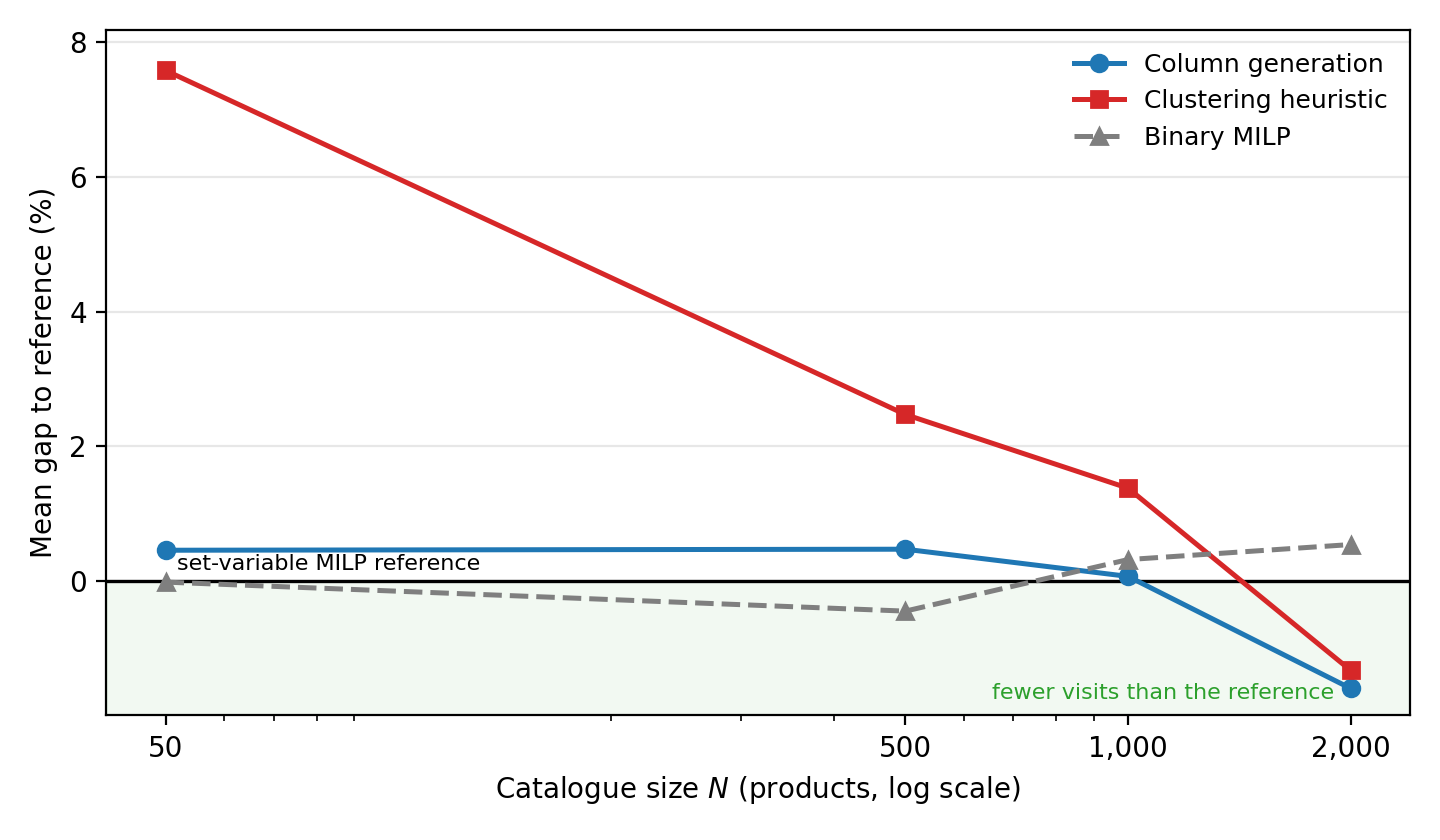
\includegraphics[width=0.86\linewidth]{Images_CSLAP/gap_vs_size_crossover.png}
\caption{Mean gap to the set-variable formulation reference against catalogue size, the reference being the horizontal line at zero, so a curve below it marks a method using fewer station visits. Both the column generation and the clustering heuristic cross the reference between 1,000 and 2,000 SKUs on this benchmark, ending $1.6\%$ and $1.5\%$ below it at 2,000, where the block holds three instances, whereas the binary MILP moves the other way and not monotonically.}
\label{fig:crossover}
\end{figure}

\textbf{Both literature baselines trail, and the objective is one plausible explanation.} Their gap to the reference widens with size, from a few percent at 50 SKUs to more than a quarter at 2,000, and neither returns fewer visits than the reference on a single instance. Objective, initialisation, constraint handling and implementation are not isolated from one another here: the baselines keep their own prescribed starts (Section~\ref{sec:init}), reach feasibility through a penalty rather than structurally, and are our own Python implementations against two commercial engines, so part of the deficit may be ours rather than theirs. What weakens with scale is the conversion rate between the surrogate and the visit count, since a swap changes that count only when it removes an order's last product from a station or carries its first to a new one, and most swaps do neither.

\textbf{The heuristic's trade of quality for time does not merely improve with scale: it reverses.} It trails at 50 SKUs, closes to within a point and a half at 1,000, and at 2,000 returns fewer visits than the reference on all three instances in under a minute against twenty. What matters is the composition of the move rather than its size: the heuristic commits a whole community to a station in one step and that community is assembled from products ordered together, so a single step can remove an order's last product from a station, whereas the genetic algorithm's crossover copies a block drawn without reference to co-occurrence and then repaired for capacity, buying no more of this objective than a single-product swap. The reversal at 2,000 SKUs rests on the same three instances as the crossing above, so we report it as observed on this benchmark rather than a general size beyond which the heuristic leads.


% =====================================================================
\section{Industrial application}\label{sec:industrial}
% =====================================================================
We validate the framework on a real warehouse, Company~A, whose instance Table~\ref{tab:instance} summarises and which operates 26 stations. Two of them, S25 and S26, are too small for a reassignment to change the visit count or to move workload, so the catalogue of $|P| = 21{,}874$ products sits on the other 24, which enter the solvers and the evaluation. Within those 24 a product keeps the location the site has already given it when it appears in at most five orders \emph{and} sits at one of the three static-shelving stations, whose slotting is not re-planned; both the threshold and the tolerance below are the site's own operating rules, not parameters we chose; a further 171 products, which survive only in orders the extract does not retain, are pinned the same way. That leaves $15{,}975$ products free to relocate and fixes $5{,}899$. Frozen products keep their slots and their workload share, so with $P^{\mathrm{fix}}_s$ the products frozen at station $s$ the optimisation runs on the residual resources $\bar\zeta_s=\zeta_s-\lvert P^{\mathrm{fix}}_s\rvert$ and $\bar T_s = T_s - \sum_{p \in P^{\mathrm{fix}}_s} L_p/V_s$, while the evaluation charges every station with its complete load on the complete order stream; the reductions below are therefore not inflated by the reduced decision pool.

\begin{table}[H]
\centering
\tbl{The Company~A instance as it enters the solvers.}
{\small\begin{tabular*}{\textwidth}{@{\extracolsep{\fill}}lr@{}}
\toprule
Quantity & Value \\
\midrule
Planning horizon & 13 weeks, 1 Sept.\ to 30 Nov.\ 2021 \\
Orders & 284{,}862 \\
Order lines over the horizon & 1{,}486{,}608 \\
Products (SKUs) & 21{,}874 \\
\quad free to relocate & 15{,}975 \\
\quad frozen in place & 5{,}899 \\
Stations, of which evaluated & 26, of which 24 \\
Movable products held per station & 8 to 2{,}575 \\
Processing rate $V_s$, lines per unit time & 6.2 to 10{,}400 \\
Legacy station load $\sum_{p} L_p/V_s$ & 0.8 to 9{,}923 \\
Workload budget $T_s$ & 110\% of the legacy load \\
\bottomrule
\end{tabular*}}
\tabnote{The two excluded stations hold 1 and 2 locations. Processing rates span three orders of magnitude because the stations use different picking technologies, which is why workload is normalised by $V_s$ and raw line counts are not comparable across stations.}
\label{tab:instance}
\end{table}

The Company~A extract is a non-public dataset. It consists of anonymised commercial operational records, order lines and station assignments, supplied by the partner company and used with its permission. It contains no personal data, and the study is non-interventional and involves no human or animal subjects, so no ethics approval was required.

Here the workload row \eqref{eq:wl} keeps the normalised form of Section~\ref{sec:model}, each station's budget $T_s$ being $110\%$ of the complete legacy load $\sum_{p} L_p/V_s$ the station carried, frozen and movable products together, with $V_s$ that station's own calibrated speed. Dividing by $V_s$ is what makes the quantity mean the same thing at every station, since the technologies differ across the range of Table~\ref{tab:instance} and a raw line count does not. The Max WL column of Table~\ref{tab:industrial} reports that load, the busiest legacy station carrying $9{,}923$. Because the budgets it is measured against still differ in size from station to station, we report alongside it each station's utilisation, its realised load as a percentage of its own legacy load, and the standard deviation of those percentages over the 24 evaluated stations; that denominator gives the legacy layout zero dispersion by construction, so the metric reads as departure from the balance the site operates.

\begin{table}[H]
\centering
\tbl{Industrial case study (Company~A, 24 evaluated stations) under a 10-hour cap. Green marks the best value in a column, orange the runner-up, red a workload violation; the shaded top row is the layout the site operates today.}
{\footnotesize\setlength{\tabcolsep}{3.5pt}\begin{tabular*}{\textwidth}{@{\extracolsep{\fill}}lrrrrrrr@{}}
\toprule
Method & Visits & Reduction (\%) & Gap vs.\ ref (\%) & Time (s) & Max WL & Util.\ SD (\%) & Viol. \\
\midrule
\rowcolor{yellow!50!black}
\textcolor{white}{Original layout (A)} & \textcolor{white}{1{,}062{,}507} & \textcolor{white}{--} & \textcolor{white}{15.81} & \textcolor{white}{0} & \textcolor{white}{9{,}923} & \cellcolor{green!80!black}\textcolor{white}{0.00} & \textcolor{white}{None} \\
Set-variable formulation & \textcolor{green!60!black}{\textbf{917{,}465}} & \textcolor{green!60!black}{\textbf{13.65}} & 0.00 & 36{,}000 & 10{,}467 & 4.48 & None \\
Binary MILP & \textcolor{orange!90!black}{\textbf{989{,}320}} & \textcolor{orange!90!black}{\textbf{6.89}} & 7.83 & 36{,}000 & 10{,}356 & \textcolor{orange!90!black}{\textbf{3.44}} & None \\
Heuristic & 996{,}448 & 6.22 & 8.61 & \cellcolor{blue!12}\textbf{790} & 10{,}915 & 27.37 & None \\
CG (station-indexed) & 1{,}000{,}844 & 5.80 & 9.09 & 36{,}000 & 10{,}074 & \textcolor{green!60!black}{\textbf{2.41}} & None \\
GA & 1{,}046{,}071 & 1.55 & 14.02 & 19{,}358 & \textcolor{red}{\textbf{10{,}972}} & 18.52 & \textcolor{red}{\textbf{WL}} \\
SA-C & 1{,}058{,}563 & 0.37 & 15.38 & 36{,}000 & 10{,}811 & 12.14 & \textcolor{red}{\textbf{WL}} \\
\bottomrule
\end{tabular*}}
\tabnote{Reduction is against the original layout, Gap vs.\ ref against the set-variable formulation. Util.\ SD is the standard deviation of each station's realised load against its own legacy load (\%). Max WL is the realised busiest-station load $\sum_{p} L_p/V_s$ of \eqref{eq:wl}, not a line count. The site tolerates up to 10\% above the complete legacy load a station carried, frozen and movable products together, and the busiest legacy station carries a load of 9,923, so its bound is 10,915. The flag marks a method exceeding its own bound at one or more stations; the check is per station, so a Max WL below 10,915 does not by itself certify feasibility. Time is the cap where a method exhausted its budget, otherwise the measured running time.}
\label{tab:industrial}
\end{table}

Table~\ref{tab:industrial} reports the outcome, where the methods separate on how they spend the workload budget before they separate on visits. The heuristic removes 6.2\% in thirteen minutes, but only by spending the tolerance in full: sixteen of the twenty-four stations end at or above $105\%$ of their legacy load, eight sit on the $110\%$ cap itself, and five are stripped below $70\%$ (Figure~\ref{fig:workload}a). Its utilisation dispersion of $27.4$ is an order of magnitude above every optimising method. The column generation removes $5.8\%$ while holding dispersion at $2.4$ and leaving headroom everywhere, and the visit counts do not separate the two: its result falls inside the spread the heuristic covers over feasible bounds, six of the eleven beating it and five not, the bound the rule itself returns among the latter (Supplementary Section~S7). A layout pinned against the cap is in any case feasible on the weeks it was fitted to and infeasible on the first week demand grows.

The community bound survives the transfer, but only a grid finds its best value. Section~\ref{sec:heuristic} sets $\beta$ from a single slot capacity, presuming interchangeable stations; here they hold between 8 and 2{,}575 movable products, and the rule applied to their mean returns $\beta=266$. That value is feasible and removes 5.7\% of the visits, yet it is not the best reachable, and feasibility is not an interval in $\beta$: $\beta=67$ and $\beta=200$ are feasible while $\beta=33$ and $\beta=133$ between them are not (Supplementary Section~S7). We therefore select $\beta$ on a seven-point grid anchored on the mean capacity, keeping the feasible layout with fewest visits. That is $\beta=333$, which gives the heuristic row of Table~\ref{tab:industrial}, its time entry charging the whole grid. The bound is not tuned: every setting above 200 is feasible and they span barely a percentage point, so the grid buys avoidance of the infeasible band. On interchangeable stations none of this arises, the rule's $\beta$ being feasible on all 29 benchmark instances.

The set-variable formulation takes the opposite position, removing 13.7\% of the station visits while every station's utilisation shift stays within $[-5.9\%, +9.6\%]$, inside the site's 10\% slack (Figure~\ref{fig:workload}b), so the deepest reduction we obtain is also deployable, although no method here returns a certified optimum. The binary MILP, on the same engine and budget, is also feasible everywhere yet carries 7.8\% more visits. The representation is the experimental treatment, engine and budget being held fixed, though the search was not instrumented, so attributing the gap specifically to the $|P| \times |S|$ repair burden the set encoding removes stays an interpretation; the synthetic family, where the two forms differ by less than 0.6\% at every scale, gives no warning of it. A benchmark of a few thousand products would have retired the reformulation as redundant.

\begin{figure}[H]
\centering
\footnotesize
(a) Clustering heuristic\par\smallskip
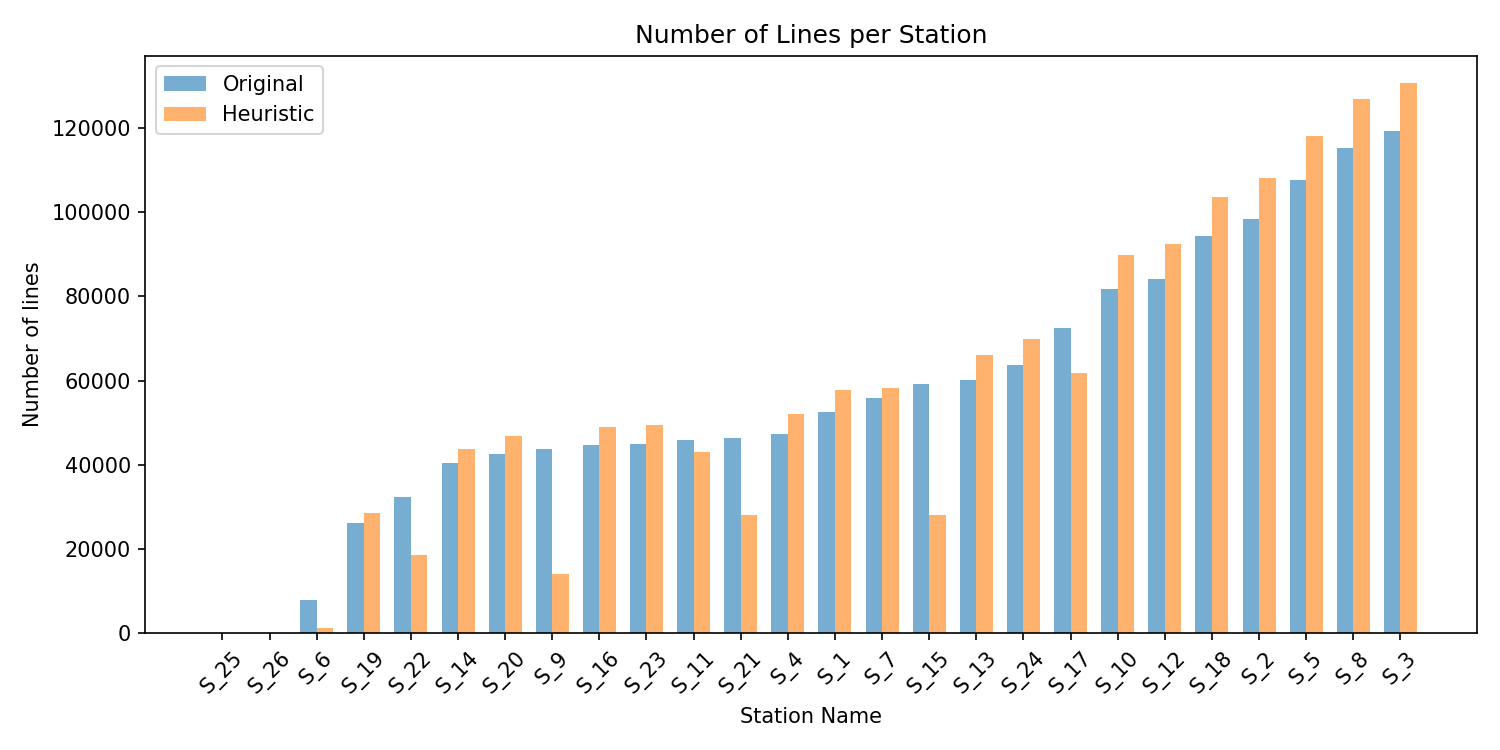
\includegraphics[width=0.46\linewidth]{Images_CSLAP/r4_number_of_lines_per_station.png}\hfill
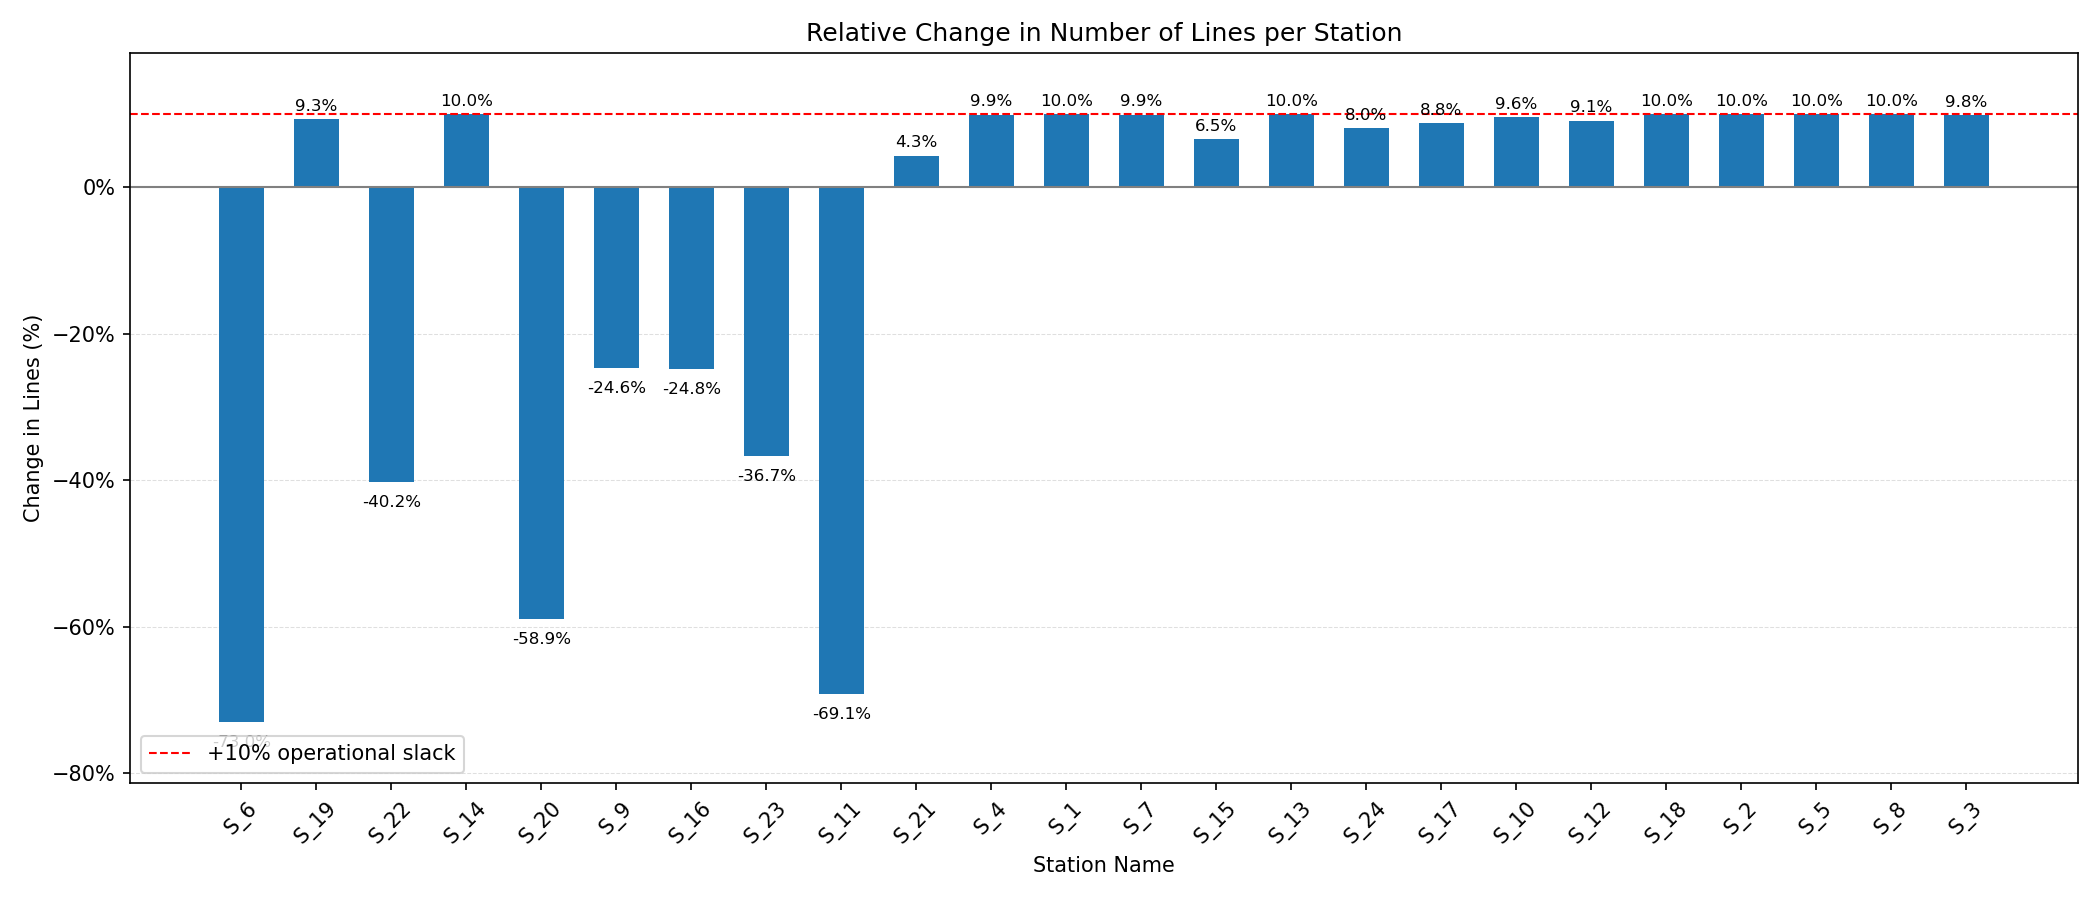
\includegraphics[width=0.46\linewidth]{Images_CSLAP/r5_pct_change_lines_per_station.png}\par\medskip
(b) Set-variable formulation\par\smallskip
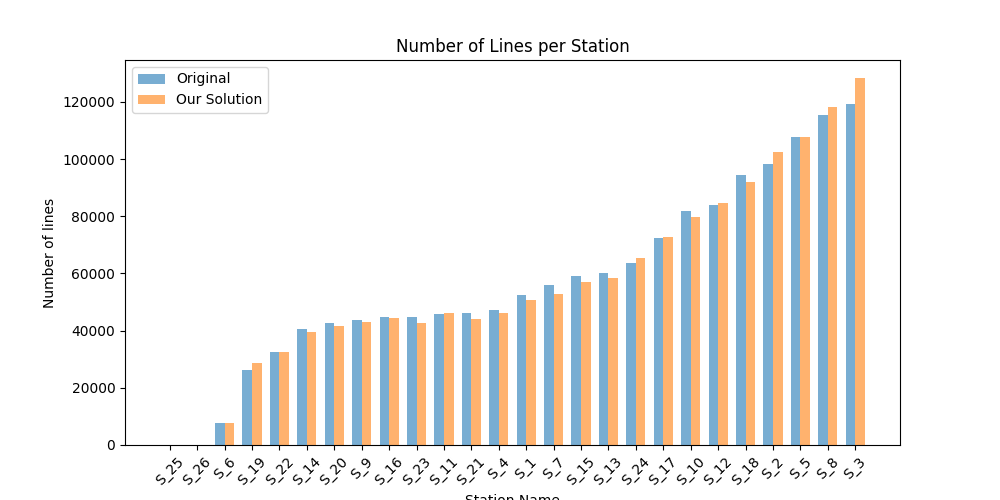
\includegraphics[width=0.46\linewidth]{Images_CSLAP/Hexaly_number_of_lines_per_station.png}\hfill
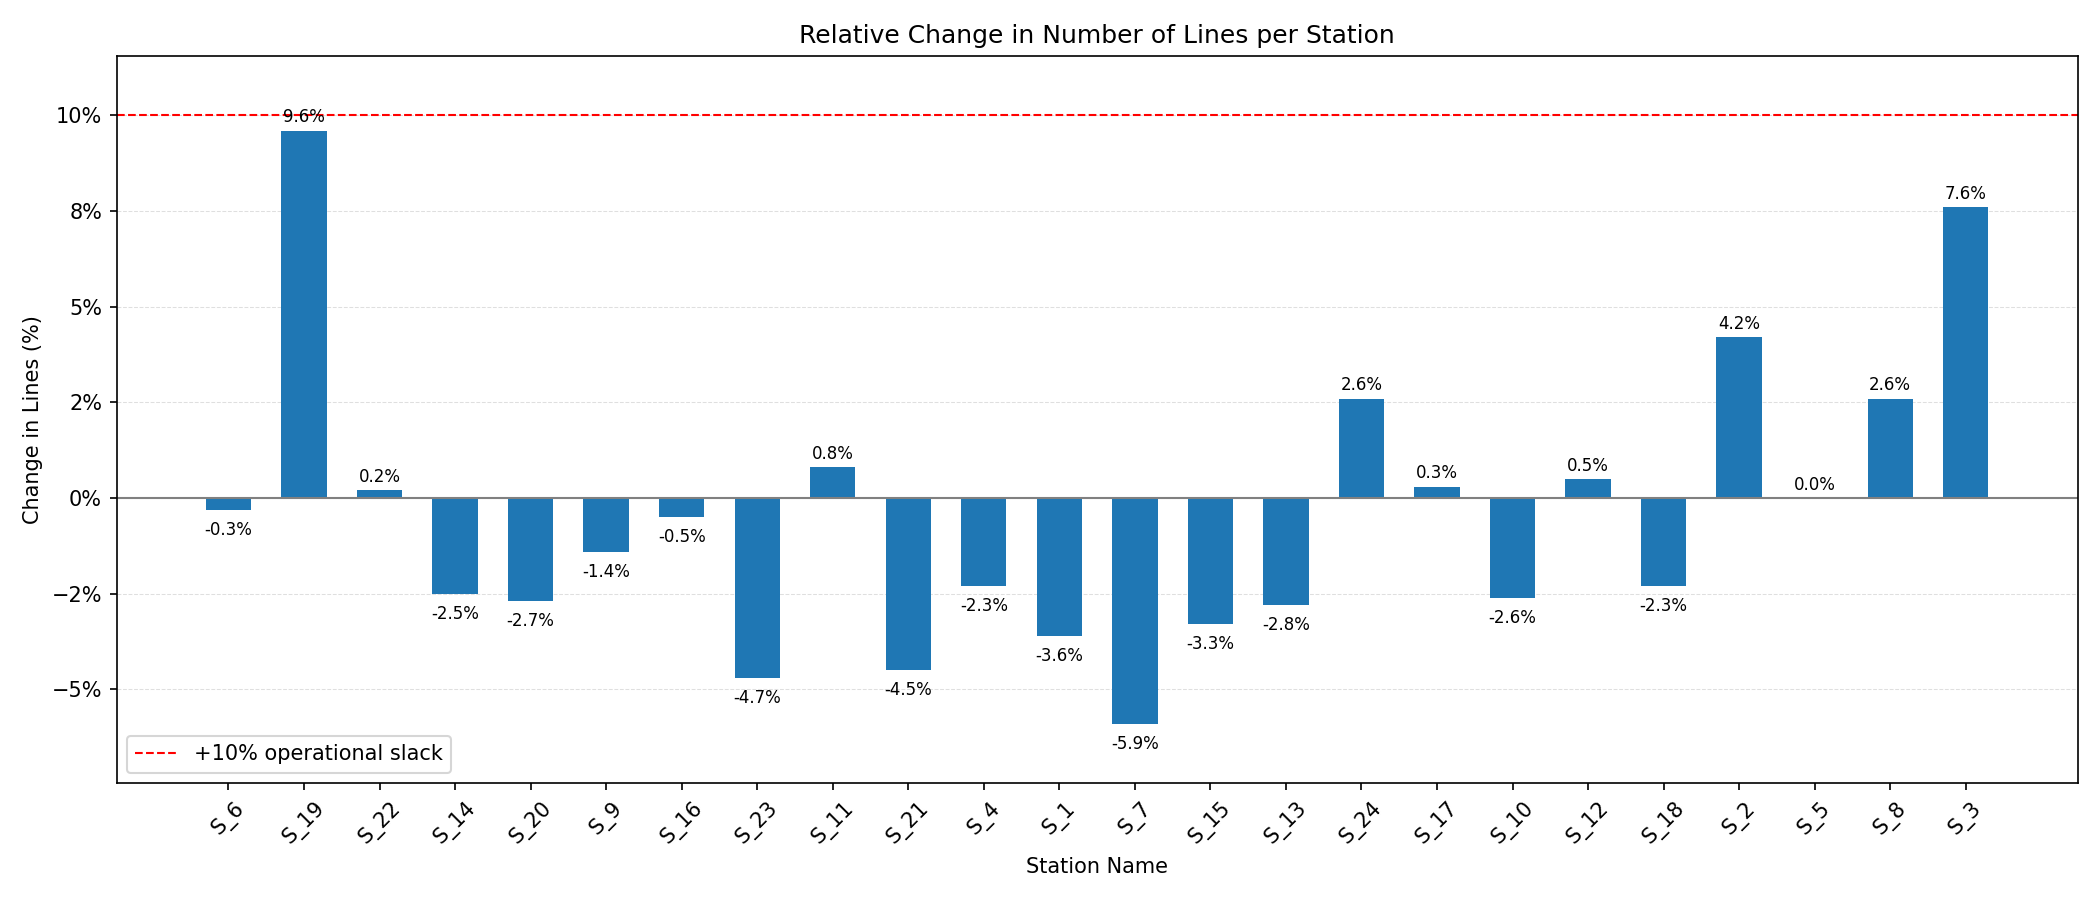
\includegraphics[width=0.46\linewidth]{Images_CSLAP/Hexaly_pt_relative_change_number_of_lines_per_station_new.png}\par\medskip
(c) Station-indexed column generation\par\smallskip
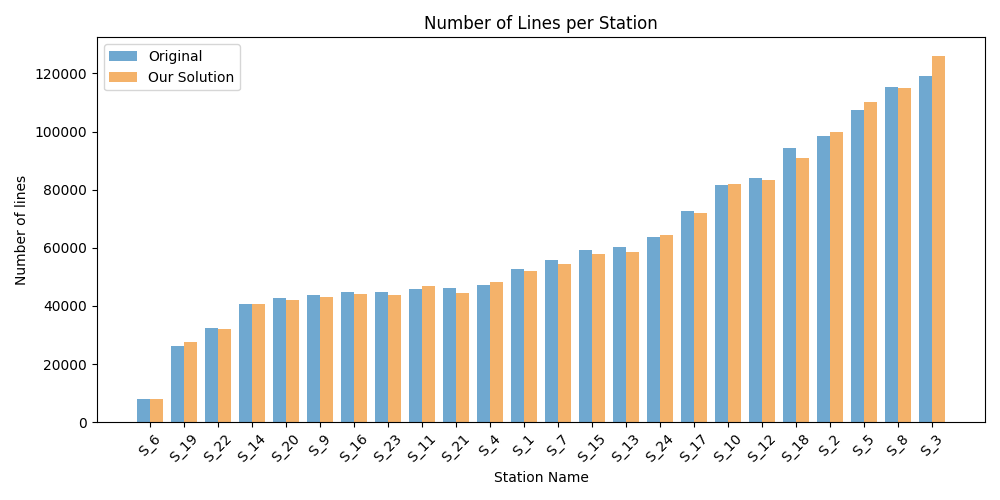
\includegraphics[width=0.46\linewidth]{Images_CSLAP/CG_SetPart_number_of_lines_per_station.png}\hfill
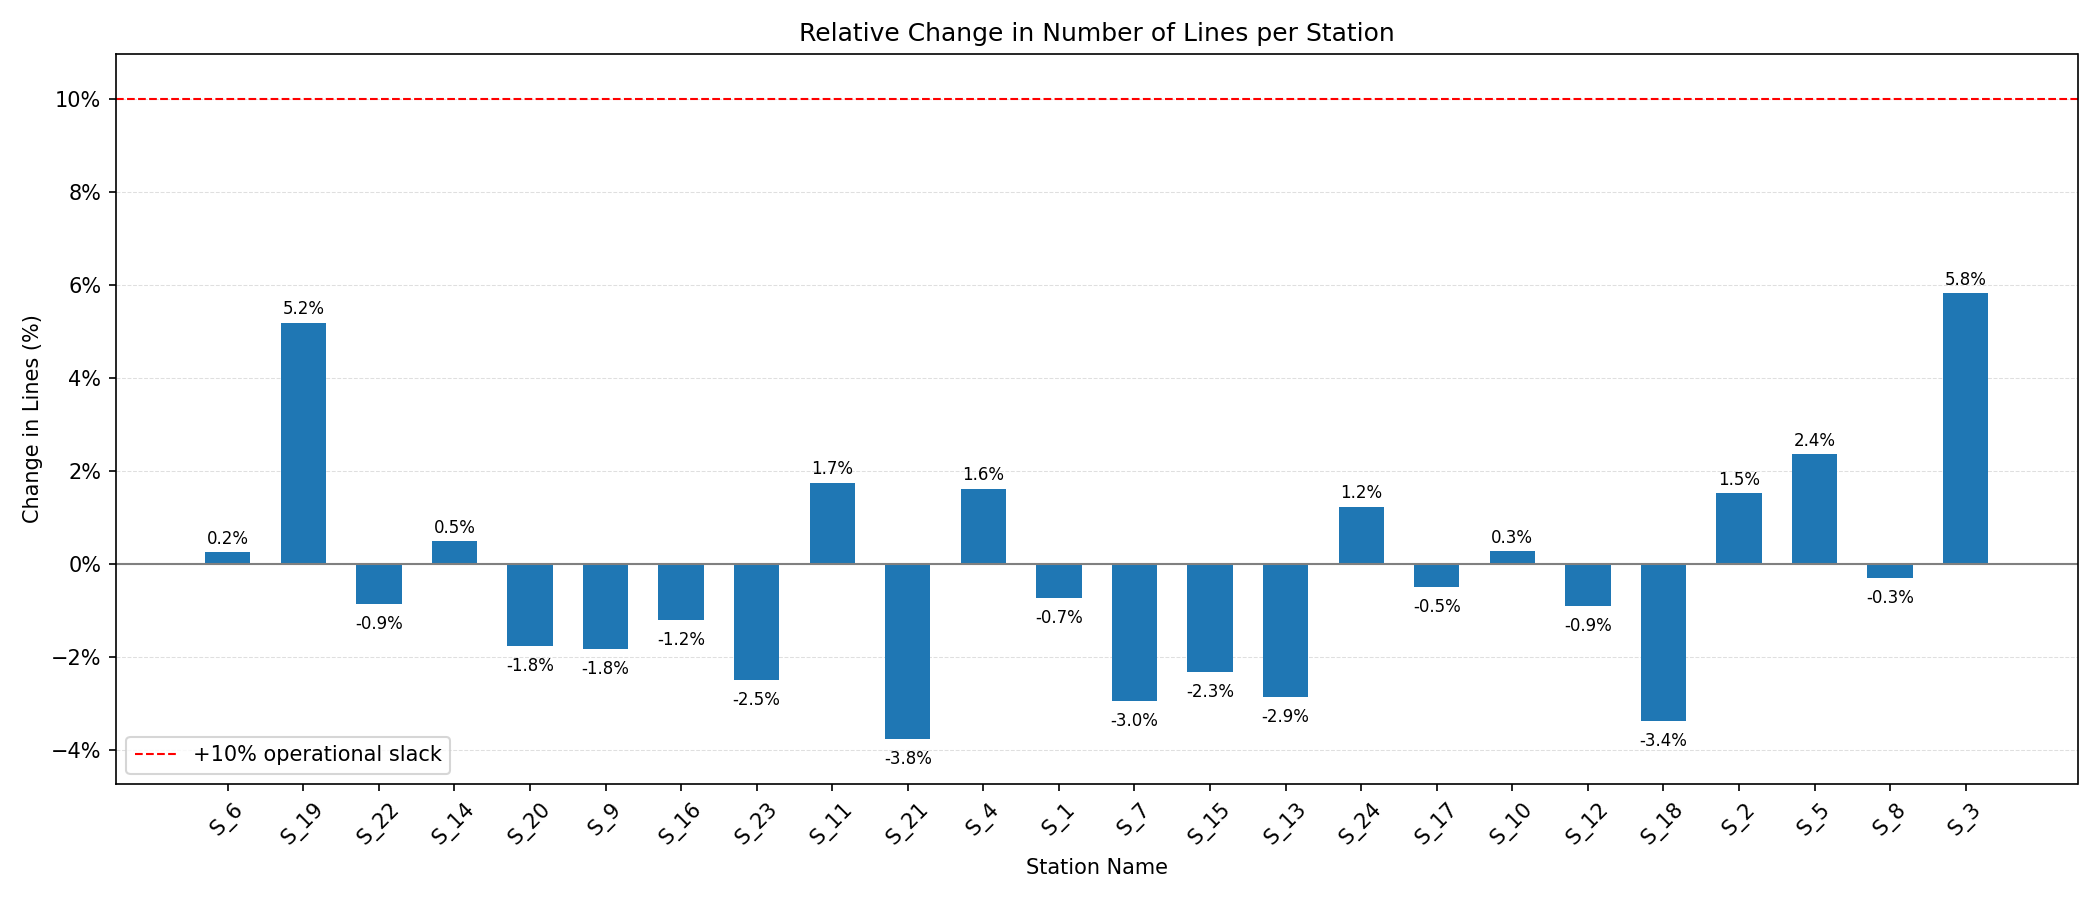
\includegraphics[width=0.46\linewidth]{Images_CSLAP/CG_SetPart_pt_relative_change_number_of_lines_per_station_new.png}
\caption{Station workload for the three deployable layouts against the original placement, with (a) the clustering heuristic, (b) the set-variable formulation and (c) the station-indexed column generation: lines per station (left) and relative change in utilisation (right). No station exceeds the site's $+10\%$ tolerance, and layout (c) tracks the legacy balance most closely. S25 and S26 are omitted from the right-hand panels, where they would show 0\% by construction.}
\label{fig:workload}
\end{figure}

The column generation ran on Company~A in its station-indexed form with the set-variable formulation's inputs, so the two solve the same constrained problem. Four elements differ from the homogeneous drive. The warm start is the live layout rather than an LPT partition. Priced bundles are installed by an ejection-style recompletion, which empties the target station, installs the bundle there and reinserts the displaced products at the stations sharing the most order weight with them. The stage budgets follow a different schedule, and a bound pass absent from the homogeneous one prices every station once more at the incumbent duals before the integer master. Supplementary Section~S5 gives both schedules. The run priced exactly throughout and used its full cap, removing 5.8\% of the visits the site incurs today. Its layout shares the set-variable solution's feasibility profile, both exceeding the raw legacy load on ten stations and both inside the site's 10\% tolerance everywhere (Figure~\ref{fig:workload}b, c). The drive produces that profile: warm-starting from the live layout keeps it near the incumbent balance, and enforcing the workload cap inside pricing means no violating bundle is generated.

The site runs about 81,700 station stops a week across the extract, so at the 6.6 to 7.4\% the layout holds on weeks it was not fitted to (Section~\ref{sec:temporal}) the expected saving is roughly 5,400 to 6,050 fewer stops per week. Each eliminated visit removes one cycle of deceleration, induction, scanning and merge, whose duration is site-specific and unmeasured here, so we state the effect per unit: for every second of per-visit cycle time the out-of-sample reduction frees 1.5 to 1.7 hours of station dwell per week. The projection is linear and ignores queueing, so a discrete-event study is needed to confirm it (Section~\ref{sec:conclusion}).

\subsection{Robustness on unseen weeks}\label{sec:temporal}
A layout is optimised once and then operated as demand evolves, so we test out of sample. The dataset spans 13 weeks, from 1 September to 30 November 2021, split on the recorded delivery date of each order: the model sees the first 10 weeks and is evaluated on the last 3, then the first 8 and the last 5, each layout compared with the original placement and with an oracle optimised on the test weeks \citep{lee2020cie, wang2020}.

This test separates two quantities the paper must not conflate. The 13.7\% of Table~\ref{tab:industrial} is in sample, the layout having been optimised on the same 13 weeks it is measured over; on unseen weeks the same method removes 6.6\% of visits on the three-week hold-out and 7.4\% on the five-week one (Table~\ref{tab:temporal}). The deployable expectation for a site re-slotting on recent history is the second pair, the first an upper bound reached only when demand does not move. The gap is not solver quality: an oracle optimised on the test weeks removes only 12.1\% and 10.2\% there, so the reduction attainable on a test period is itself below the in-sample figure, which is consistent with substantial demand shift between the fitting and evaluation windows. Read against that oracle the fitted layouts retain 55\% and 72\% of the available reduction, the share rising with the evaluation window, though the splits vary training and evaluation windows together, so the effect of each is not separated. Recent history is therefore sufficient for a durable gain here, though that stability may not carry to more volatile assortments.

\begin{table}[H]
\centering
\tbl{Out-of-sample station-visit performance on held-out weeks.}
{\begin{tabular*}{\textwidth}{@{\extracolsep{\fill}}llrrr@{}}
\toprule
Test period & Layout (training period) & Total visits & Mean visits & Reduction (\%) \\
\midrule
\multirow{3}{*}{Last 3 weeks}
 & Original placement & 265{,}876 & 4.052 & -- \\
 & Optimised on first 10 weeks & 248{,}358 & 3.785 & 6.6 \\
 & Oracle (optimised on last 3 weeks) & 233{,}728 & 3.562 & 12.1 \\
\midrule
\multirow{3}{*}{Last 5 weeks}
 & Original placement & 423{,}593 & 3.926 & -- \\
 & Optimised on first 8 weeks & 392{,}318 & 3.636 & 7.4 \\
 & Oracle (optimised on last 5 weeks) & 380{,}356 & 3.525 & 10.2 \\
\bottomrule
\end{tabular*}}
\tabnote{All layouts are produced by the set-variable formulation under the 10-hour cap of Table~\ref{tab:industrial}, the training and evaluation windows changing together between the two splits. Mean visits is total visits divided by the number of orders in the test period, that is the average number of stations an order visits. Reduction is against the original placement on the same test window, so it is measured out of sample for the fitted layouts and in sample for the oracle.}
\label{tab:temporal}
\end{table}

\subsection{Bounded reassignment}\label{sec:reassign}
An established facility cannot absorb a disruptive re-slotting wave \citep{chabot2024reassignment}, so we bound how many products may move. With $s'(p)$ the legacy station of $p$, one constraint
\begin{equation}
\sum_{p \in P} x_{p,\,s'(p)} \ \ge\ |P| - k
\label{eq:reassign}
\end{equation}
limits the relocated products to at most $k$. Nothing else changes and the legacy layout stays feasible for every $k$, so the model has a solution whatever budget the site sets; the cap also admits a column-generation form, stated in Supplementary Section~S9 but not run here. We solve it with the set-variable formulation for $k \in \{250, 500, 1000, 2000, 5000\}$ under a one-hour limit each, against the legacy layout ($k=0$) and the full re-optimisation (Table~\ref{tab:reassign}).

\begin{table}[H]
\centering
\tbl{Bounded-reassignment trade-off on the industrial instance.}
{\small\begin{tabular*}{\textwidth}{@{\extracolsep{\fill}}lrrrrr@{}}
\toprule
Relocation cap & \% catalogue & Total visits & Reduction & \% of full benefit & WL-viol.\ stations \\
\midrule
Legacy ($k=0$) & 0\% & 1{,}062{,}507 & -- & -- & 0 \\
$k=250$        & 1.1\% & 1{,}061{,}302 & 1{,}205 & 0.8\% & 0 \\
$k=500$        & 2.3\% & 1{,}060{,}120 & 2{,}387 & 1.6\% & 0 \\
$k=1{,}000$    & 4.6\% & 1{,}056{,}412 & 6{,}095 & 4.2\% & 0 \\
$k=2{,}000$    & 9.1\% & 1{,}049{,}730 & 12{,}777 & 8.8\% & 0 \\
$k=5{,}000$    & 22.9\% & 1{,}034{,}735 & 27{,}772 & 19.2\% & 0 \\
Full re-opt.   & --     & 917{,}465 & 145{,}042 & 100\% & 0 \\
\bottomrule
\end{tabular*}}
\tabnote{``\% catalogue'' is $k$ as a share of all 21,874 products, of which only 15,975 can relocate. ``\% of full benefit'' is the reduction as a share of the 145,042 visits removed by the full re-optimisation.}
\label{tab:reassign}
\end{table}

Bounded re-slotting returns benefit sub-proportionally to effort at every cap: at $k = 5{,}000$, which is $31.3\%$ of the $15{,}975$ movable products, the layout captures $19.2\%$ of the available reduction, about 5.6 visits per relocated product against at least $145{,}042/15{,}975 \approx 9.1$ for the full re-optimisation, and no cap shows an inflection point at which a small subset of moves captures a disproportionate share. The objective explains the asymmetry: a visit disappears only when an order loses its last product at a station, so relocating part of a co-ordered group yields nothing until the remainder follows. We cannot separate that structural reading from an effect of the search budget: every bounded run exhausted its hour against the ten hours of the full re-optimisation, and none converged, so how much of the shortfall a longer run would recover is not measured here. Every point of the trade-off is nonetheless deployable, all stations staying within capacity and workload and close to their legacy loads, so a site can set its relocation budget against available labour.

% =====================================================================
\section{Managerial insights}\label{sec:managerial}
% =====================================================================
The results yield four implications for warehouse operations.

\textbf{Track station visits as a slotting indicator.} Each diversion generates mechanical queueing and handling delay, so stops per order expose congestion that a distance metric hides.

\textbf{Read the labour effect as a planning figure, not a saving.} Build it on the out-of-sample reduction: a layout measured on the weeks it was fitted to removes 13.7\% of visits, but on unseen weeks the figure is 6.6 to 7.4\% (Section~\ref{sec:temporal}), and only the latter describes what a site will operate with. The freed dwell scales with a site's own per-visit cycle time assuming no queue forms, so a site should substitute its measured cycle time and commission a discrete-event study before treating the figure as realised.

\textbf{Match the tool to the decision, and to the warehouse.} Where stations differ in geometry and speed, as Company~A's do, the set-variable formulation gives the best layout we obtain within capacity; where they are interchangeable the choice shifts with catalogue size, the ranking reversing between 1,000 and 2,000 SKUs without a size we can fix. Where the priority is minimal disturbance to an engineered balance, choose the column generation, which held the workload limit in every experiment. The clustering heuristic suits a layout needed quickly or often, on two conditions: it disturbs the existing distribution of work the most, so a site should check station-level loads against its own tolerance and not the cap alone, and where stations differ widely in capacity its community bound has to be chosen on a short grid rather than read off the rule (Section~\ref{sec:industrial}).

\textbf{Run the layout as a lifecycle rather than a project.} A layout optimised on the most recent 8 to 10 weeks retains $55\%$ and $72\%$ of the reduction an oracle could obtain on the following weeks, the share rising with the length of the evaluation window. We did not vary the re-optimisation frequency itself, so treat windows of this length as a starting point for a re-slotting cycle rather than as a validated cadence, while bounded reassignment keeps each cycle non-disruptive by moving only as many products as the workforce can handle and holding every station within capacity and workload at each cap of Table~\ref{tab:reassign}.

% =====================================================================
\section{Conclusions and research perspectives}\label{sec:conclusion}
% =====================================================================
We posed the correlated storage location assignment problem for automated pick-and-pass warehouses with station visits as the objective and hard capacity and workload limits, replacing the travel-distance objective that correlated storage models inherit from manual picking. On a real 21,874-product warehouse the reformulated model removes 13.7\% of station visits in sample and 6.6 to 7.4\% on weeks it was not fitted to, in both cases within every station limit, and a relocation cap lets a site take that gain in stages rather than in one disruptive wave. The three strategies then divide the ground between them. The set-variable formulation gives the deepest reduction we obtain and is the form we would deploy; the binary encoding of the same model, run as a representation control on the same engine, carries 7.8\% more visits at industrial scale while the two stay within 0.6\% of each other on the synthetic benchmark. We attribute that divergence to the decision representation rather than to solver technology, though the mechanism is not instrumented here, and it is the clearest sign in our results that a benchmark of a few thousand products cannot settle the choice of representation. A set-partitioning column generation, driven as a price-and-complete matheuristic, never breaches a workload cap, improves the live industrial layout by 5.8\% while disturbing the engineered balance least, and overtakes the reference between 1,000 and 2,000 products on this benchmark, on three instances at the larger size. The clustering heuristic is the fast fallback, reaching a lower visit count than the reference at 2,000 products in under a minute against twenty. On the industrial site it removes 6.2\% in thirteen minutes, but spends the whole workload tolerance and leaves most stations at their cap, so it earns its place where a layout is needed quickly rather than where a ten-hour budget is available.

Four tracks extend the work, two on the method. Dual stabilisation \citep{dumerle1999stabilized, wentges1997weighted} is the first, and Section~\ref{sec:cgbound} gives the measured reason for preferring it to a stronger formulation: the master never priced out inside the cap, so the bound is limited by how far the dual iteration got rather than by the relaxation's strength, and reaching $z_{\mathrm{LP}}$ would turn the matheuristic reading into certified gaps. A fuller account would isolate the drive's operators by ablation and carry an adaptive large neighbourhood search and an open-source constraint-programming model \citep{ropke2006alns, perron2023cpsat} as further baselines, the latter measuring the cost to a practitioner without a commercial licence.

Two concern the model. The first is product geometry: replacing the unit count of a station's capacity with a per-product footprint $f_p$ in \eqref{eq:cap} would admit three-dimensional packing limits without changing the structure of the programme, and the same extension covers duplicating a high-demand product across stations, which the single-station assumption excludes. The second is the visit-to-throughput link: we balance workload, which lowers expected queueing, but do not model the queue, and feeding the optimised layouts into a discrete-event simulation would convert the planning figures of Section~\ref{sec:managerial} into measured throughput and open the way to stochastic demand and real-time routing. What these layouts are worth in throughput rather than stops is the question we leave open.

% ---------------------------------------------------------------------
% BACK MATTER (order per the IJSS:O&L Original Article specification)
% ---------------------------------------------------------------------
\section*{Author contributions}
All authors were involved in the conception, design and modelling of the framework. Ermal Belul developed the software, analysed the empirical data and drafted the manuscript; Marwane Bouznif, Dritan Nace and Antoine Jouglet critically revised it for intellectual content. All authors approved the final version and agree to be accountable for the work.

\section*{Acknowledgements}
The authors thank the operational teams at Company~A for the dataset and their insight into the picking process, and Savoye and the Universit\'{e} de technologie de Compi\`{e}gne for hosting the work.

\section*{Funding details}
This work was supported by the Association Nationale de la Recherche et de la Technologie (ANRT) under a CIFRE doctoral grant in partnership with Savoye.

\section*{Disclosure of interest}
The authors report there are no competing interests to declare.

\section*{Declaration of generative AI use}
During the preparation of this work the authors used a generative AI assistant to refine language and improve readability. The authors subsequently reviewed and edited the content and take full responsibility for the published article.

\section*{Data availability statement}
This journal applies the Taylor \& Francis ``share upon reasonable request'' data sharing policy. Both synthetic instance families are openly available, the 29 benchmark and 80 calibration instances, each with the generator, station counts and seeds that produced them, together with the per-instance column-generation convergence record of Supplementary Section~S8, at \href{https://anonymous.4open.science/r/Anonymized_Export_CSLAP_v2-01BC/README.md}{this repository}. The Company~A dataset and the dated extract behind Table~\ref{tab:temporal} cannot be made public because of commercial confidentiality, and may be requested from the authors under reasonable operational conditions. Hexaly and IBM CPLEX depend on commercial licences we cannot redistribute; the model statements and settings needed to rebuild the methods on another solver are given in Sections~\ref{sec:model}, \ref{sec:cg} and~\ref{sec:experiments}.


% ---------------------------------------------------------------------
\section*{Notes on contributors}
\noindent\textit{Ermal Belul} is a doctoral candidate at the Universit\'{e} de technologie de Compi\`{e}gne, Heudiasyc laboratory, working under an industrial (CIFRE) agreement with Savoye. His research concerns decision-support models for warehouse storage assignment and intralogistics planning under uncertainty.

\medskip
\noindent\textit{Marwane Bouznif} is a machine learning and optimisation engineer at Savoye. He holds a doctorate from the Universit\'{e} de Grenoble (2012) on constant-time generic algorithms for combinatorial problems in rotagraphs and fasciagraphs. His current work applies operations research and machine learning to automated warehousing, including sorting, robot fleet sizing and storage assignment.

\medskip
\noindent\textit{Dritan Nace} is Professor at the Universit\'{e} de technologie de Compi\`{e}gne and a member of the Heudiasyc laboratory (UMR CNRS 7253), where he leads the SCOP research team. His work addresses operations research and network optimisation, in particular robust and survivable network design, resilient routing, and fair resource allocation.

\medskip
\noindent\textit{Antoine Jouglet} is Professor at the Universit\'{e} de technologie de Compi\`{e}gne and a member of the Heudiasyc laboratory (UMR CNRS 7253), in the SCOP research team. His work addresses combinatorial optimisation and scheduling, with a focus on dominance rules, exact and hybrid solution methods, and their application to industrial logistics problems.

% ---------------------------------------------------------------------
% References (APA via apacite)
% ---------------------------------------------------------------------
\bibliographystyle{apacite}
\bibliography{IJSSOL_CSLAP_v1}

\end{document}
